\documentclass[twoside]{book}

% Packages required by doxygen
\usepackage{fixltx2e}
\usepackage{calc}
\usepackage{doxygen}
\usepackage[export]{adjustbox} % also loads graphicx
\usepackage{graphicx}
\usepackage[utf8]{inputenc}
\usepackage{makeidx}
\usepackage{multicol}
\usepackage{multirow}
\PassOptionsToPackage{warn}{textcomp}
\usepackage{textcomp}
\usepackage[nointegrals]{wasysym}
\usepackage[table]{xcolor}

% Font selection
\usepackage[T1]{fontenc}
\usepackage[scaled=.90]{helvet}
\usepackage{courier}
\usepackage{amssymb}
\usepackage{sectsty}
\renewcommand{\familydefault}{\sfdefault}
\allsectionsfont{%
  \fontseries{bc}\selectfont%
  \color{darkgray}%
}
\renewcommand{\DoxyLabelFont}{%
  \fontseries{bc}\selectfont%
  \color{darkgray}%
}
\newcommand{\+}{\discretionary{\mbox{\scriptsize$\hookleftarrow$}}{}{}}

% Page & text layout
\usepackage{geometry}
\geometry{%
  a4paper,%
  top=2.5cm,%
  bottom=2.5cm,%
  left=2.5cm,%
  right=2.5cm%
}
\tolerance=750
\hfuzz=15pt
\hbadness=750
\setlength{\emergencystretch}{15pt}
\setlength{\parindent}{0cm}
\setlength{\parskip}{3ex plus 2ex minus 2ex}
\makeatletter
\renewcommand{\paragraph}{%
  \@startsection{paragraph}{4}{0ex}{-1.0ex}{1.0ex}{%
    \normalfont\normalsize\bfseries\SS@parafont%
  }%
}
\renewcommand{\subparagraph}{%
  \@startsection{subparagraph}{5}{0ex}{-1.0ex}{1.0ex}{%
    \normalfont\normalsize\bfseries\SS@subparafont%
  }%
}
\makeatother

% Headers & footers
\usepackage{fancyhdr}
\pagestyle{fancyplain}
\fancyhead[LE]{\fancyplain{}{\bfseries\thepage}}
\fancyhead[CE]{\fancyplain{}{}}
\fancyhead[RE]{\fancyplain{}{\bfseries\leftmark}}
\fancyhead[LO]{\fancyplain{}{\bfseries\rightmark}}
\fancyhead[CO]{\fancyplain{}{}}
\fancyhead[RO]{\fancyplain{}{\bfseries\thepage}}
\fancyfoot[LE]{\fancyplain{}{}}
\fancyfoot[CE]{\fancyplain{}{}}
\fancyfoot[RE]{\fancyplain{}{\bfseries\scriptsize Generated by Doxygen }}
\fancyfoot[LO]{\fancyplain{}{\bfseries\scriptsize Generated by Doxygen }}
\fancyfoot[CO]{\fancyplain{}{}}
\fancyfoot[RO]{\fancyplain{}{}}
\renewcommand{\footrulewidth}{0.4pt}
\renewcommand{\chaptermark}[1]{%
  \markboth{#1}{}%
}
\renewcommand{\sectionmark}[1]{%
  \markright{\thesection\ #1}%
}

% Indices & bibliography
\usepackage{natbib}
\usepackage[titles]{tocloft}
\setcounter{tocdepth}{3}
\setcounter{secnumdepth}{5}
\makeindex

% Hyperlinks (required, but should be loaded last)
\usepackage{ifpdf}
\ifpdf
  \usepackage[pdftex,pagebackref=true]{hyperref}
\else
  \usepackage[ps2pdf,pagebackref=true]{hyperref}
\fi
\hypersetup{%
  colorlinks=true,%
  linkcolor=blue,%
  citecolor=blue,%
  unicode%
}

% Custom commands
\newcommand{\clearemptydoublepage}{%
  \newpage{\pagestyle{empty}\cleardoublepage}%
}

\usepackage{caption}
\captionsetup{labelsep=space,justification=centering,font={bf},singlelinecheck=off,skip=4pt,position=top}

%===== C O N T E N T S =====

\begin{document}

% Titlepage & ToC
\hypersetup{pageanchor=false,
             bookmarksnumbered=true,
             pdfencoding=unicode
            }
\pagenumbering{roman}
\begin{titlepage}
\vspace*{7cm}
\begin{center}%
{\Large M\+PX Thunder Krakens \\[1ex]\large R1 }\\
\vspace*{1cm}
{\large Generated by Doxygen 1.8.11}\\
\end{center}
\end{titlepage}
\clearemptydoublepage
\tableofcontents
\clearemptydoublepage
\pagenumbering{arabic}
\hypersetup{pageanchor=true}

%--- Begin generated contents ---
\chapter{Class Index}
\section{Class List}
Here are the classes, structs, unions and interfaces with brief descriptions\+:\begin{DoxyCompactList}
\item\contentsline{section}{\hyperlink{structfunction__name}{function\+\_\+name} }{\pageref{structfunction__name}}{}
\end{DoxyCompactList}

\chapter{File Index}
\section{File List}
Here is a list of all files with brief descriptions\+:\begin{DoxyCompactList}
\item\contentsline{section}{include/\hyperlink{string_8h}{string.\+h} \\*Many usefull functions that used for handling string }{\pageref{string_8h}}{}
\item\contentsline{section}{include/core/\hyperlink{serial_8h}{serial.\+h} \\*Serial -\/ Header }{\pageref{serial_8h}}{}
\item\contentsline{section}{lib/\hyperlink{string_8c}{string.\+c} \\*Many usefull functions that used for handling string }{\pageref{string_8c}}{}
\item\contentsline{section}{modules/\hyperlink{errno_8h}{errno.\+h} \\*This file contains the type of errors. The error can be from invalid paramter passed to a function, or invalid input format }{\pageref{errno_8h}}{}
\item\contentsline{section}{modules/r1/\hyperlink{r1_8c}{r1.\+c} \\*The commandhander and functions associations for Module R1 }{\pageref{r1_8c}}{}
\item\contentsline{section}{modules/r1/\hyperlink{r1_8h}{r1.\+h} \\*The commandhander and functions associations for Module R1 }{\pageref{r1_8h}}{}
\item\contentsline{section}{modules/r1/\hyperlink{sys__clock_8c}{sys\+\_\+clock.\+c} \\*The main file that manipulates and controls the system\textquotesingle{}s clock }{\pageref{sys__clock_8c}}{}
\item\contentsline{section}{modules/r1/\hyperlink{sys__clock_8h}{sys\+\_\+clock.\+h} \\*The main file that manipulates and controls the system\textquotesingle{}s clock }{\pageref{sys__clock_8h}}{}
\item\contentsline{section}{modules/r2/\hyperlink{pcb_8c}{pcb.\+c} \\*The Process Control Block }{\pageref{pcb_8c}}{}
\item\contentsline{section}{modules/r2/\hyperlink{pcb_8h}{pcb.\+h} \\*The Process Control Block }{\pageref{pcb_8h}}{}
\item\contentsline{section}{modules/r2/\hyperlink{pcb__comm_8c}{pcb\+\_\+comm.\+c} \\*The main functions that manipulate the P\+CB }{\pageref{pcb__comm_8c}}{}
\item\contentsline{section}{modules/r2/\hyperlink{pcb__comm_8h}{pcb\+\_\+comm.\+h} \\*The main functions that manipulate the P\+CB }{\pageref{pcb__comm_8h}}{}
\end{DoxyCompactList}

\chapter{Class Documentation}
\hypertarget{structfunction__name}{}\section{function\+\_\+name Struct Reference}
\label{structfunction__name}\index{function\+\_\+name@{function\+\_\+name}}
\subsection*{Public Attributes}
\begin{DoxyCompactItemize}
\item 
char $\ast$ {\bfseries name\+Str}\hypertarget{structfunction__name_a7a94f7f31542a15b63160b6b213e0bcb}{}\label{structfunction__name_a7a94f7f31542a15b63160b6b213e0bcb}

\item 
int($\ast$ {\bfseries function} )(int argc, char $\ast$$\ast$argv)\hypertarget{structfunction__name_ad80214b3eea6c438c13ff5461c5350ab}{}\label{structfunction__name_ad80214b3eea6c438c13ff5461c5350ab}

\item 
char $\ast$ {\bfseries usage}\hypertarget{structfunction__name_a30f593e52febda0cc9d9703b9015fb0f}{}\label{structfunction__name_a30f593e52febda0cc9d9703b9015fb0f}

\item 
char $\ast$ {\bfseries help}\hypertarget{structfunction__name_ac0f73e570d7d03a9f378a70e6d4d5632}{}\label{structfunction__name_ac0f73e570d7d03a9f378a70e6d4d5632}

\end{DoxyCompactItemize}


The documentation for this struct was generated from the following file\+:\begin{DoxyCompactItemize}
\item 
modules/r1/\hyperlink{r1_8h}{r1.\+h}\end{DoxyCompactItemize}

\chapter{File Documentation}
\hypertarget{serial_8h}{}\section{include/core/serial.h File Reference}
\label{serial_8h}\index{include/core/serial.\+h@{include/core/serial.\+h}}


Serial -\/ Header.  


\subsection*{Macros}
\begin{DoxyCompactItemize}
\item 
\#define {\bfseries C\+O\+M1}~0x3f8\hypertarget{serial_8h_a00dbb3ab1c59e14699be9393693e2248}{}\label{serial_8h_a00dbb3ab1c59e14699be9393693e2248}

\item 
\#define {\bfseries C\+O\+M2}~0x2f8\hypertarget{serial_8h_a435e02f194c24c9b0e00d7cd27a1704e}{}\label{serial_8h_a435e02f194c24c9b0e00d7cd27a1704e}

\item 
\#define {\bfseries C\+O\+M3}~0x3e8\hypertarget{serial_8h_abbed02672431595364c5dd35809303a6}{}\label{serial_8h_abbed02672431595364c5dd35809303a6}

\item 
\#define {\bfseries C\+O\+M4}~0x2e8\hypertarget{serial_8h_a595cabb01568ba641574d24546d99c6b}{}\label{serial_8h_a595cabb01568ba641574d24546d99c6b}

\item 
\#define {\bfseries Without\+Echo}~0\hypertarget{serial_8h_a99c15aced355f0ca133b05cf46a7ff28}{}\label{serial_8h_a99c15aced355f0ca133b05cf46a7ff28}

\item 
\#define {\bfseries With\+Echo}~1\hypertarget{serial_8h_afddb5e7f7cc4e3632a18609dabf32628}{}\label{serial_8h_afddb5e7f7cc4e3632a18609dabf32628}

\end{DoxyCompactItemize}
\subsection*{Functions}
\begin{DoxyCompactItemize}
\item 
int {\bfseries init\+\_\+serial} (int device)\hypertarget{serial_8h_a7078c07ff8b2c48780558549a8f7cf90}{}\label{serial_8h_a7078c07ff8b2c48780558549a8f7cf90}

\item 
int {\bfseries serial\+\_\+println} (const char $\ast$msg)\hypertarget{serial_8h_a3514f7abff236a4e00a6c46021ce5e22}{}\label{serial_8h_a3514f7abff236a4e00a6c46021ce5e22}

\item 
int {\bfseries serial\+\_\+print} (const char $\ast$msg)\hypertarget{serial_8h_a995827efcd4dcfb780c9fbb9645410a4}{}\label{serial_8h_a995827efcd4dcfb780c9fbb9645410a4}

\item 
int {\bfseries set\+\_\+serial\+\_\+out} (int device)\hypertarget{serial_8h_ae97b87ee1f57c687e7fca6f9958e03ef}{}\label{serial_8h_ae97b87ee1f57c687e7fca6f9958e03ef}

\item 
int {\bfseries set\+\_\+serial\+\_\+in} (int device)\hypertarget{serial_8h_a3f4008da5feabfb7e086f6673a81104b}{}\label{serial_8h_a3f4008da5feabfb7e086f6673a81104b}

\item 
void \hyperlink{serial_8h_aca81fe61abc40b171257825521578e6c}{get\+\_\+input\+\_\+line} (char $\ast$buffer, const int buffer\+\_\+size, const int b\+With\+Echo)
\begin{DoxyCompactList}\small\item\em get\+\_\+input\+\_\+line. \end{DoxyCompactList}\end{DoxyCompactItemize}


\subsection{Detailed Description}
Serial -\/ Header. 

\begin{DoxyAuthor}{Author}
Thunder Krakens 
\end{DoxyAuthor}
\begin{DoxyDate}{Date}
February 2nd, 2016 
\end{DoxyDate}
\begin{DoxyVersion}{Version}
R1 
\end{DoxyVersion}


\subsection{Function Documentation}
\index{serial.\+h@{serial.\+h}!get\+\_\+input\+\_\+line@{get\+\_\+input\+\_\+line}}
\index{get\+\_\+input\+\_\+line@{get\+\_\+input\+\_\+line}!serial.\+h@{serial.\+h}}
\subsubsection[{\texorpdfstring{get\+\_\+input\+\_\+line(char $\ast$buffer, const int buffer\+\_\+size, const int b\+With\+Echo)}{get_input_line(char *buffer, const int buffer_size, const int bWithEcho)}}]{\setlength{\rightskip}{0pt plus 5cm}void get\+\_\+input\+\_\+line (
\begin{DoxyParamCaption}
\item[{char $\ast$}]{buffer, }
\item[{const int}]{buffer\+\_\+size, }
\item[{const int}]{b\+With\+Echo}
\end{DoxyParamCaption}
)}\hypertarget{serial_8h_aca81fe61abc40b171257825521578e6c}{}\label{serial_8h_aca81fe61abc40b171257825521578e6c}


get\+\_\+input\+\_\+line. 

Description\+: Get user\textquotesingle{}s input from keyborad. 
\begin{DoxyParams}{Parameters}
{\em buffer} & -\/ The pointer to the buffer where store the user\textquotesingle{}s input. \\
\hline
{\em buffer\+\_\+size} & -\/ The size of that buffer. \\
\hline
{\em b\+With\+Echo} & -\/ With echo or not \\
\hline
\end{DoxyParams}
\begin{DoxyReturn}{Returns}
V\+O\+ID 
\end{DoxyReturn}

\hypertarget{string_8h}{}\section{include/string.h File Reference}
\label{string_8h}\index{include/string.\+h@{include/string.\+h}}


Many usefull functions that used for handling string.  


{\ttfamily \#include $<$system.\+h$>$}\\*
Include dependency graph for string.\+h\+:
\nopagebreak
\begin{figure}[H]
\begin{center}
\leavevmode
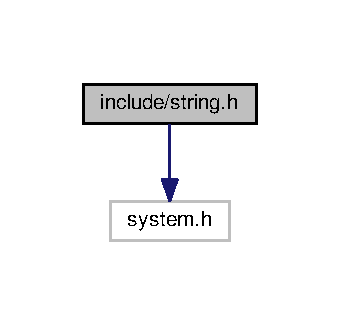
\includegraphics[width=163pt]{string_8h__incl}
\end{center}
\end{figure}
This graph shows which files directly or indirectly include this file\+:
\nopagebreak
\begin{figure}[H]
\begin{center}
\leavevmode
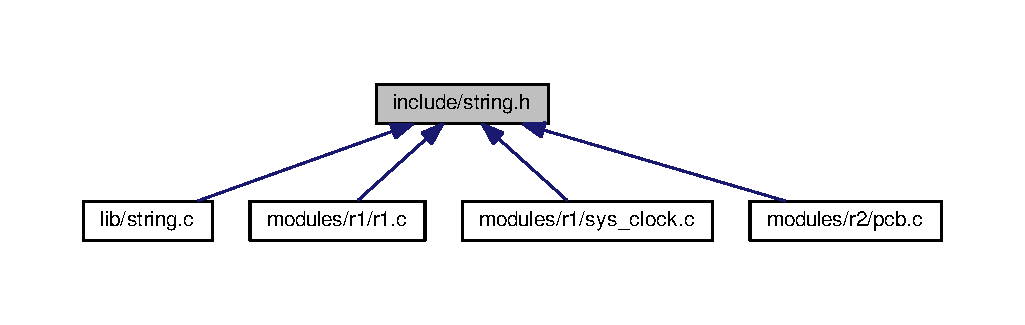
\includegraphics[width=350pt]{string_8h__dep__incl}
\end{center}
\end{figure}
\subsection*{Functions}
\begin{Indent}{\bf isspace.}\par
{\em Identifies if its space


\begin{DoxyParams}{Parameters}
{\em A} & constant character\\
\hline
\end{DoxyParams}
\begin{DoxyReturn}{Returns}
1 if it is space, otherwise return 0. 
\end{DoxyReturn}
}\begin{DoxyCompactItemize}
\item 
int {\bfseries isspace} (const char $\ast$c)\hypertarget{string_8h_a0f3d37d605e9e6d4fc1853ff9d4b91bf}{}\label{string_8h_a0f3d37d605e9e6d4fc1853ff9d4b91bf}

\end{DoxyCompactItemize}
\end{Indent}
\begin{Indent}{\bf memset.}\par
{\em Sets region of memory


\begin{DoxyParams}{Parameters}
{\em s} & destination \\
\hline
{\em c} & byte to write \\
\hline
{\em n} & count \\
\hline
\end{DoxyParams}
\begin{DoxyReturn}{Returns}
the pointer to the memory space. 
\end{DoxyReturn}
}\begin{DoxyCompactItemize}
\item 
void $\ast$ {\bfseries memset} (void $\ast$s, int c, size\+\_\+t n)\hypertarget{string_8h_ace6ee45c30e71865e6eb635200379db9}{}\label{string_8h_ace6ee45c30e71865e6eb635200379db9}

\end{DoxyCompactItemize}
\end{Indent}
\begin{Indent}{\bf \+: strcpy.}\par
{\em Copies one string to another.


\begin{DoxyParams}{Parameters}
{\em s1} & Destination string \\
\hline
{\em s2} & Source string\\
\hline
\end{DoxyParams}
\begin{DoxyReturn}{Returns}
pointer to the destination String 
\end{DoxyReturn}
}\begin{DoxyCompactItemize}
\item 
char $\ast$ {\bfseries strcpy} (char $\ast$s1, const char $\ast$s2)\hypertarget{string_8h_a1eb9cae61e6a6282c28dbc298ef7297e}{}\label{string_8h_a1eb9cae61e6a6282c28dbc298ef7297e}

\end{DoxyCompactItemize}
\end{Indent}
\begin{Indent}{\bf strcat.}\par
{\em Concatenate the contents of one string onto another.


\begin{DoxyParams}{Parameters}
{\em s1} & Destination string \\
\hline
{\em s2} & Source string \\
\hline
\end{DoxyParams}
\begin{DoxyReturn}{Returns}
pointer to destination String 
\end{DoxyReturn}
}\begin{DoxyCompactItemize}
\item 
char $\ast$ {\bfseries strcat} (char $\ast$s1, const char $\ast$s2)\hypertarget{string_8h_a8908188ae9fc2f05d993257ef001d553}{}\label{string_8h_a8908188ae9fc2f05d993257ef001d553}

\end{DoxyCompactItemize}
\end{Indent}
\begin{Indent}{\bf \+: strlen.}\par
{\em Returns the length of a string.


\begin{DoxyParams}{Parameters}
{\em s} & String input.\\
\hline
\end{DoxyParams}
\begin{DoxyReturn}{Returns}
count Length of the String 
\end{DoxyReturn}
}\begin{DoxyCompactItemize}
\item 
int {\bfseries strlen} (const char $\ast$s)\hypertarget{string_8h_a2dee044e4e667b5b789b493abd21cfa4}{}\label{string_8h_a2dee044e4e667b5b789b493abd21cfa4}

\end{DoxyCompactItemize}
\end{Indent}
\begin{Indent}{\bf \+: strcmp.}\par
{\em String comparison.


\begin{DoxyParams}{Parameters}
{\em s1} & First string to use for the compare. \\
\hline
{\em s2} & Second string to use for the compare.\\
\hline
\end{DoxyParams}
\begin{DoxyReturn}{Returns}
whether they are the same or not. 
\end{DoxyReturn}
}\begin{DoxyCompactItemize}
\item 
int {\bfseries strcmp} (const char $\ast$s1, const char $\ast$s2)\hypertarget{string_8h_a11bd144d7d44914099a3aeddf1c8567d}{}\label{string_8h_a11bd144d7d44914099a3aeddf1c8567d}

\end{DoxyCompactItemize}
\end{Indent}
\begin{Indent}{\bf strtok.}\par
{\em Split string into tokens.


\begin{DoxyParams}{Parameters}
{\em s1} & String \\
\hline
{\em s2} & Delimiter \\
\hline
\end{DoxyParams}
\begin{DoxyReturn}{Returns}
the pointer to the token. 
\end{DoxyReturn}
}\begin{DoxyCompactItemize}
\item 
char $\ast$ {\bfseries strtok} (char $\ast$s1, const char $\ast$s2)\hypertarget{string_8h_af1a867dcea42fc1215d0eddf19283ef3}{}\label{string_8h_af1a867dcea42fc1215d0eddf19283ef3}

\end{DoxyCompactItemize}
\end{Indent}
\begin{Indent}{\bf \+: atoi.}\par
{\em Convert an A\+S\+C\+II string to an integer.


\begin{DoxyParams}{Parameters}
{\em s} & String.\\
\hline
\end{DoxyParams}
\begin{DoxyReturn}{Returns}
The converted integer. 
\end{DoxyReturn}
}\begin{DoxyCompactItemize}
\item 
int {\bfseries atoi} (const char $\ast$s)\hypertarget{string_8h_a30670a60464f77af17dfb353353d6df8}{}\label{string_8h_a30670a60464f77af17dfb353353d6df8}

\end{DoxyCompactItemize}
\end{Indent}
\begin{Indent}{\bf \+: sprintf.}\par
{\em Generate a formatted string.

\%\mbox{[}-\/x\mbox{]}c output a character, \textquotesingle{}-\/\textquotesingle{} -\/ align right, x -\/ the output width

\%\mbox{[}-\/x\mbox{]}s output a string, \textquotesingle{}-\/\textquotesingle{} -\/ align right, x -\/ the output width

\%\mbox{[}\{-\/,+\}x\mbox{]}d output a character, \textquotesingle{}-\/\textquotesingle{} -\/ align right, \textquotesingle{}+\textquotesingle{} -\/ align right and display \textquotesingle{}+\textquotesingle{} sign, x -\/ the output width

\%\mbox{[}-\/x\mbox{]}X (capital \textquotesingle{}X\textquotesingle{}) output a hexadecimal number, \textquotesingle{}-\/\textquotesingle{} -\/ align right, x -\/ the output width

note\+: Output width will be ignored if width is smaller than actual length.


\begin{DoxyParams}{Parameters}
{\em str} & -\/ Output string. \\
\hline
{\em format} & -\/ The format of the string. \\
\hline
{\em ...} & -\/ All of the additional parameters. \\
\hline
\end{DoxyParams}
\begin{DoxyReturn}{Returns}
vsprintf(str, format, ap) -\/ Return the string with its format and pointer. 
\end{DoxyReturn}
}\begin{DoxyCompactItemize}
\item 
int {\bfseries sprintf} (char $\ast$str, const char $\ast$format,...)\hypertarget{string_8h_a3082155ec11e7229f7a20439b31a169e}{}\label{string_8h_a3082155ec11e7229f7a20439b31a169e}

\end{DoxyCompactItemize}
\end{Indent}
\begin{Indent}{\bf printf.}\par
{\em Print out a formatted string.

\%\mbox{[}-\/x\mbox{]}c output a character, \textquotesingle{}-\/\textquotesingle{} -\/ align right, x -\/ the output width

\%\mbox{[}-\/x\mbox{]}s output a string, \textquotesingle{}-\/\textquotesingle{} -\/ align right, x -\/ the output width

\%\mbox{[}\{-\/,+\}x\mbox{]}d output a character, \textquotesingle{}-\/\textquotesingle{} -\/ align right, \textquotesingle{}+\textquotesingle{} -\/ align right and display \textquotesingle{}+\textquotesingle{} sign, x -\/ the output width

\%\mbox{[}-\/x\mbox{]}X (capital \textquotesingle{}X\textquotesingle{}) output a hexadecimal number, \textquotesingle{}-\/\textquotesingle{} -\/ align right, x -\/ the output width

note\+: Output width will be ignored if width is smaller than actual length.


\begin{DoxyParams}{Parameters}
{\em str} & -\/ Output string. \\
\hline
{\em format} & -\/ The format of the string. \\
\hline
{\em ...} & -\/ All of the additional parameters. \\
\hline
\end{DoxyParams}
\begin{DoxyReturn}{Returns}
vsprintf(str, format, ap) -\/ Return the string with its format and pointer. 
\end{DoxyReturn}
}\begin{DoxyCompactItemize}
\item 
int {\bfseries printf} (const char $\ast$format,...)\hypertarget{string_8h_a98631211a4a8aee62f572375d5b637be}{}\label{string_8h_a98631211a4a8aee62f572375d5b637be}

\end{DoxyCompactItemize}
\end{Indent}


\subsection{Detailed Description}
Many usefull functions that used for handling string. 

\begin{DoxyAuthor}{Author}
Thunder Krakens 
\end{DoxyAuthor}
\begin{DoxyDate}{Date}
February 2nd, 2016 
\end{DoxyDate}
\begin{DoxyVersion}{Version}
R1 
\end{DoxyVersion}

\hypertarget{serial_8c}{}\section{kernel/core/serial.c File Reference}
\label{serial_8c}\index{kernel/core/serial.\+c@{kernel/core/serial.\+c}}


Serial.  


{\ttfamily \#include $<$stdint.\+h$>$}\\*
{\ttfamily \#include $<$string.\+h$>$}\\*
{\ttfamily \#include $<$core/io.\+h$>$}\\*
{\ttfamily \#include $<$core/serial.\+h$>$}\\*
Include dependency graph for serial.\+c\+:
\nopagebreak
\begin{figure}[H]
\begin{center}
\leavevmode
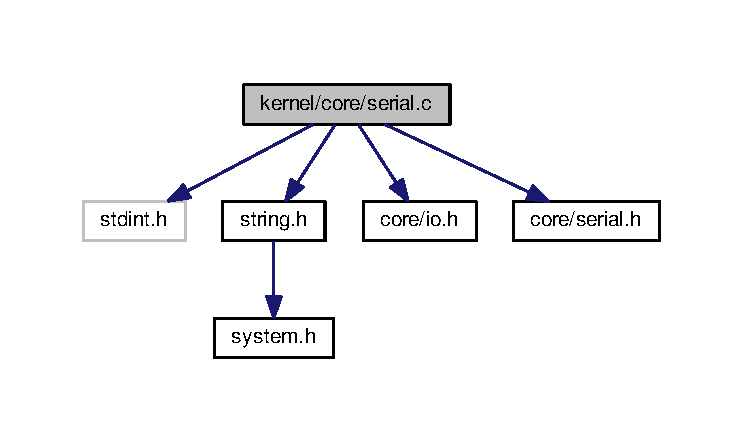
\includegraphics[width=350pt]{serial_8c__incl}
\end{center}
\end{figure}
\subsection*{Macros}
\begin{DoxyCompactItemize}
\item 
\#define {\bfseries N\+O\+\_\+\+E\+R\+R\+OR}~0\hypertarget{serial_8c_a258bb72419ef143530a2f8f55e7d57af}{}\label{serial_8c_a258bb72419ef143530a2f8f55e7d57af}

\item 
\#define {\bfseries E\+S\+C\+\_\+\+K\+EY}~27\hypertarget{serial_8c_a9b4f59fc9220530978f12905fe51b1d0}{}\label{serial_8c_a9b4f59fc9220530978f12905fe51b1d0}

\item 
\#define {\bfseries B\+R\+A\+C\+K\+E\+T\+\_\+\+K\+EY}~91\hypertarget{serial_8c_ac54e60a8f1f354c38e128f13125afa71}{}\label{serial_8c_ac54e60a8f1f354c38e128f13125afa71}

\item 
\#define {\bfseries E\+N\+T\+E\+R\+\_\+\+K\+EY}~13\hypertarget{serial_8c_afba17fd121bcd7abc852f1ae1f3abb58}{}\label{serial_8c_afba17fd121bcd7abc852f1ae1f3abb58}

\item 
\#define {\bfseries B\+A\+C\+K\+S\+P\+A\+C\+E\+\_\+\+K\+EY}~127\hypertarget{serial_8c_a899616376b07e20f03dbae5894465a92}{}\label{serial_8c_a899616376b07e20f03dbae5894465a92}

\item 
\#define {\bfseries D\+E\+L\+\_\+\+K\+E\+Y\+\_\+\+S\+E\+Q\+\_\+3}~51\hypertarget{serial_8c_a3ba2d95bba1e70b0f8bc3204686534a6}{}\label{serial_8c_a3ba2d95bba1e70b0f8bc3204686534a6}

\item 
\#define {\bfseries D\+E\+L\+\_\+\+K\+E\+Y\+\_\+\+S\+E\+Q\+\_\+4}~126\hypertarget{serial_8c_a64bd4e101a2323b02d6b47172b6e41ba}{}\label{serial_8c_a64bd4e101a2323b02d6b47172b6e41ba}

\item 
\#define {\bfseries U\+P\+\_\+\+A\+R\+R\+OW}~65\hypertarget{serial_8c_ad315ce436b88e78c266532e4714dd197}{}\label{serial_8c_ad315ce436b88e78c266532e4714dd197}

\item 
\#define {\bfseries D\+O\+W\+N\+\_\+\+A\+R\+R\+OW}~66\hypertarget{serial_8c_a5b1eca6358420b8748a151949d3119fa}{}\label{serial_8c_a5b1eca6358420b8748a151949d3119fa}

\item 
\#define {\bfseries R\+I\+G\+H\+T\+\_\+\+A\+R\+R\+OW}~67\hypertarget{serial_8c_a9ed2533108b634266a6261c8f37e4fc0}{}\label{serial_8c_a9ed2533108b634266a6261c8f37e4fc0}

\item 
\#define {\bfseries L\+E\+F\+T\+\_\+\+A\+R\+R\+OW}~68\hypertarget{serial_8c_ae78ccf44cb7970752cbfeb22e6a66d14}{}\label{serial_8c_ae78ccf44cb7970752cbfeb22e6a66d14}

\end{DoxyCompactItemize}
\subsection*{Functions}
\begin{DoxyCompactItemize}
\item 
int {\bfseries init\+\_\+serial} (int device)\hypertarget{serial_8c_a7078c07ff8b2c48780558549a8f7cf90}{}\label{serial_8c_a7078c07ff8b2c48780558549a8f7cf90}

\item 
int {\bfseries serial\+\_\+println} (const char $\ast$msg)\hypertarget{serial_8c_a3514f7abff236a4e00a6c46021ce5e22}{}\label{serial_8c_a3514f7abff236a4e00a6c46021ce5e22}

\item 
int {\bfseries serial\+\_\+print} (const char $\ast$msg)\hypertarget{serial_8c_a995827efcd4dcfb780c9fbb9645410a4}{}\label{serial_8c_a995827efcd4dcfb780c9fbb9645410a4}

\item 
int {\bfseries set\+\_\+serial\+\_\+out} (int device)\hypertarget{serial_8c_ae97b87ee1f57c687e7fca6f9958e03ef}{}\label{serial_8c_ae97b87ee1f57c687e7fca6f9958e03ef}

\item 
int {\bfseries set\+\_\+serial\+\_\+in} (int device)\hypertarget{serial_8c_a3f4008da5feabfb7e086f6673a81104b}{}\label{serial_8c_a3f4008da5feabfb7e086f6673a81104b}

\end{DoxyCompactItemize}
\begin{Indent}{\bf Move\+Cursor\+Backchar.}\par
{\em Move the cursor back for specific times.


\begin{DoxyParams}{Parameters}
{\em num} & The number of times that needs to move back. \\
\hline
\end{DoxyParams}
\begin{DoxyReturn}{Returns}
V\+O\+ID 
\end{DoxyReturn}
}\end{Indent}
\begin{Indent}{\bf Print\+Stars.}\par
{\em Print out the \textquotesingle{}$\ast$\textquotesingle{} for specific times.


\begin{DoxyParams}{Parameters}
{\em num} & The number of times that needs to print. \\
\hline
\end{DoxyParams}
\begin{DoxyReturn}{Returns}
V\+O\+ID 
\end{DoxyReturn}
}\end{Indent}
\begin{Indent}{\bf Echo\+Input.}\par
{\em Decides to print out the original string or stars.


\begin{DoxyParams}{Parameters}
{\em Input\+Str} & The string, \\
\hline
{\em b\+With\+Echo} & Turn on the echo or not. \\
\hline
\end{DoxyParams}
}\end{Indent}
\begin{Indent}{\bf get\+\_\+input\+\_\+line}\par
{\em Get user\textquotesingle{}s input from keyborad.


\begin{DoxyParams}{Parameters}
{\em buffer} & The pointer to the buffer where store the user\textquotesingle{}s input. \\
\hline
{\em buffer\+\_\+size} & The size of that buffer. \\
\hline
{\em b\+With\+Echo} & With echo or not\\
\hline
\end{DoxyParams}
\begin{DoxyReturn}{Returns}
V\+O\+ID 
\end{DoxyReturn}
}\begin{DoxyCompactItemize}
\item 
void {\bfseries get\+\_\+input\+\_\+line} (char $\ast$buffer, const int buffer\+\_\+size, const int b\+With\+Echo)\hypertarget{serial_8c_aca81fe61abc40b171257825521578e6c}{}\label{serial_8c_aca81fe61abc40b171257825521578e6c}

\end{DoxyCompactItemize}
\end{Indent}
\subsection*{Variables}
\begin{DoxyCompactItemize}
\item 
int {\bfseries serial\+\_\+port\+\_\+out} = 0\hypertarget{serial_8c_adbb2c18b0aaab5c1927a6f674768a710}{}\label{serial_8c_adbb2c18b0aaab5c1927a6f674768a710}

\item 
int {\bfseries serial\+\_\+port\+\_\+in} = 0\hypertarget{serial_8c_a1a756238531fc5bf1096f89dc18e835e}{}\label{serial_8c_a1a756238531fc5bf1096f89dc18e835e}

\end{DoxyCompactItemize}


\subsection{Detailed Description}
Serial. 

\begin{DoxyAuthor}{Author}
Thunder Krakens 
\end{DoxyAuthor}
\begin{DoxyDate}{Date}
February 2nd, 2016 
\end{DoxyDate}
\begin{DoxyVersion}{Version}
R1 
\end{DoxyVersion}

\hypertarget{string_8c}{}\section{lib/string.c File Reference}
\label{string_8c}\index{lib/string.\+c@{lib/string.\+c}}


Many usefull functions that used for handling string.  


{\ttfamily \#include $<$system.\+h$>$}\\*
{\ttfamily \#include $<$core/serial.\+h$>$}\\*
{\ttfamily \#include $<$string.\+h$>$}\\*
Include dependency graph for string.\+c\+:\nopagebreak
\begin{figure}[H]
\begin{center}
\leavevmode
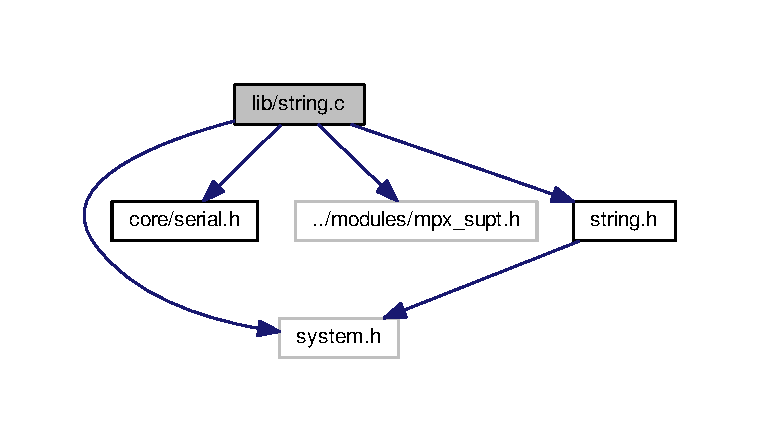
\includegraphics[width=229pt]{string_8c__incl}
\end{center}
\end{figure}
\subsection*{Functions}
\begin{Indent}{\bf strlen.}\par
{\em Returns the length of a string.


\begin{DoxyParams}{Parameters}
{\em s} & String input.\\
\hline
\end{DoxyParams}
\begin{DoxyReturn}{Returns}
count Length of the String 
\end{DoxyReturn}
}\begin{DoxyCompactItemize}
\item 
int \hyperlink{string_8c_a2dee044e4e667b5b789b493abd21cfa4}{strlen} (const char $\ast$s)
\end{DoxyCompactItemize}
\end{Indent}
\begin{Indent}{\bf strcpy.}\par
{\em Copies one string to another.


\begin{DoxyParams}{Parameters}
{\em s1} & Destination string \\
\hline
{\em s2} & Source string\\
\hline
\end{DoxyParams}
\begin{DoxyReturn}{Returns}
pointer to the destination String 
\end{DoxyReturn}
}\begin{DoxyCompactItemize}
\item 
char $\ast$ \hyperlink{string_8c_a1eb9cae61e6a6282c28dbc298ef7297e}{strcpy} (char $\ast$s1, const char $\ast$s2)
\end{DoxyCompactItemize}
\end{Indent}
\begin{Indent}{\bf atoi.}\par
{\em Convert an A\+S\+C\+II string to an integer.


\begin{DoxyParams}{Parameters}
{\em s} & String.\\
\hline
\end{DoxyParams}
\begin{DoxyReturn}{Returns}
The converted integer. 
\end{DoxyReturn}
}\begin{DoxyCompactItemize}
\item 
int \hyperlink{string_8c_a30670a60464f77af17dfb353353d6df8}{atoi} (const char $\ast$s)
\end{DoxyCompactItemize}
\end{Indent}
\begin{Indent}{\bf strcmp.}\par
{\em String comparison.


\begin{DoxyParams}{Parameters}
{\em s1} & First string to use for the compare. \\
\hline
{\em s2} & Second string to use for the compare.\\
\hline
\end{DoxyParams}
\begin{DoxyReturn}{Returns}
whether they are the same or not. 
\end{DoxyReturn}
}\begin{DoxyCompactItemize}
\item 
int \hyperlink{string_8c_a11bd144d7d44914099a3aeddf1c8567d}{strcmp} (const char $\ast$s1, const char $\ast$s2)
\end{DoxyCompactItemize}
\end{Indent}
\begin{Indent}{\bf Parse\+Padding.}\par
{\em Parse the number for padding.

(static -\/ Only can be access within this file).


\begin{DoxyParams}{Parameters}
{\em str} & Paddling String \\
\hline
{\em width} & Paddling Width \\
\hline
{\em Dec\+Width} & Width of decimal part. \\
\hline
{\em b\+Is\+Right} & Is align right. \\
\hline
{\em b\+Has\+Sign} & Has + / -\/.\\
\hline
\end{DoxyParams}
\begin{DoxyReturn}{Returns}
b\+Is\+Valid Returns the validity. 
\end{DoxyReturn}
}\end{Indent}
\begin{Indent}{\bf Add\+Pad.}\par
{\em Add a certain number of paddings (static -\/ Only can be access within this file).


\begin{DoxyParams}{Parameters}
{\em str} & In string. \\
\hline
{\em count} & Number of whitespace.\\
\hline
\end{DoxyParams}
\begin{DoxyReturn}{Returns}
V\+O\+ID 
\end{DoxyReturn}
}\end{Indent}
\begin{Indent}{\bf Nibble\+To\+Char}\par
{\em convert a nibble into a single hexadecimal (static -\/ Only can be access within this file)


\begin{DoxyParams}{Parameters}
{\em value} & The value of the nibble\\
\hline
\end{DoxyParams}
\begin{DoxyReturn}{Returns}
the character of the Hexadecimal number if valid, otherwise, return \textquotesingle{}$\ast$\textquotesingle{}. 
\end{DoxyReturn}
}\end{Indent}
\begin{Indent}{\bf bytes\+To\+Hex\+String.}\par
{\em Convert bytes into a hexadecimal string (static -\/ Only can be access within this file).


\begin{DoxyParams}{Parameters}
{\em Out\+Str} & Output string. \\
\hline
{\em Value} & The value of bytes.\\
\hline
\end{DoxyParams}
\begin{DoxyReturn}{Returns}
V\+O\+ID 
\end{DoxyReturn}
}\end{Indent}
\begin{Indent}{\bf vsprintf.}\par
{\em The actual function that perform the \char`\"{}printf\char`\"{} and \char`\"{}sprintf\char`\"{} function (static -\/ Only can be access within this file).


\begin{DoxyParams}{Parameters}
{\em str} & Output string. \\
\hline
{\em format} & The format of the string. \\
\hline
{\em ap} & the pointer of the first additional parameter.\\
\hline
\end{DoxyParams}
\begin{DoxyReturn}{Returns}
0 
\end{DoxyReturn}
}\end{Indent}
\begin{Indent}{\bf sprintf.}\par
{\em Generate a formatted string.

\%\mbox{[}-\/x\mbox{]}c output a character, \textquotesingle{}-\/\textquotesingle{} -\/ align right, x -\/ the output width

\%\mbox{[}-\/x\mbox{]}s output a string, \textquotesingle{}-\/\textquotesingle{} -\/ align right, x -\/ the output width

\%\mbox{[}\{-\/,+\}x\mbox{]}d output a character, \textquotesingle{}-\/\textquotesingle{} -\/ align right, \textquotesingle{}+\textquotesingle{} -\/ align right and display \textquotesingle{}+\textquotesingle{} sign, x -\/ the output width

\%\mbox{[}-\/x\mbox{]}X (capital \textquotesingle{}X\textquotesingle{}) output a hexadecimal number, \textquotesingle{}-\/\textquotesingle{} -\/ align right, x -\/ the output width

note\+: Output width will be ignored if width is smaller than actual length.


\begin{DoxyParams}{Parameters}
{\em str} & -\/ Output string. \\
\hline
{\em format} & -\/ The format of the string. \\
\hline
{\em ...} & -\/ All of the additional parameters. \\
\hline
\end{DoxyParams}
\begin{DoxyReturn}{Returns}
vsprintf(str, format, ap) -\/ Return the string with its format and pointer. 
\end{DoxyReturn}
}\begin{DoxyCompactItemize}
\item 
int \hyperlink{string_8c_a3082155ec11e7229f7a20439b31a169e}{sprintf} (char $\ast$str, const char $\ast$format,...)
\end{DoxyCompactItemize}
\end{Indent}
\begin{Indent}{\bf printf.}\par
{\em Print out a formatted string.

\%\mbox{[}-\/x\mbox{]}c output a character, \textquotesingle{}-\/\textquotesingle{} -\/ align right, x -\/ the output width

\%\mbox{[}-\/x\mbox{]}s output a string, \textquotesingle{}-\/\textquotesingle{} -\/ align right, x -\/ the output width

\%\mbox{[}\{-\/,+\}x\mbox{]}d output a character, \textquotesingle{}-\/\textquotesingle{} -\/ align right, \textquotesingle{}+\textquotesingle{} -\/ align right and display \textquotesingle{}+\textquotesingle{} sign, x -\/ the output width

\%\mbox{[}-\/x\mbox{]}X (capital \textquotesingle{}X\textquotesingle{}) output a hexadecimal number, \textquotesingle{}-\/\textquotesingle{} -\/ align right, x -\/ the output width

note\+: Output width will be ignored if width is smaller than actual length.


\begin{DoxyParams}{Parameters}
{\em str} & -\/ Output string. \\
\hline
{\em format} & -\/ The format of the string. \\
\hline
{\em ...} & -\/ All of the additional parameters. \\
\hline
\end{DoxyParams}
\begin{DoxyReturn}{Returns}
vsprintf(str, format, ap) -\/ Return the string with its format and pointer. 
\end{DoxyReturn}
}\begin{DoxyCompactItemize}
\item 
int \hyperlink{string_8c_a98631211a4a8aee62f572375d5b637be}{printf} (const char $\ast$format,...)
\item 
char $\ast$ \hyperlink{string_8c_a8908188ae9fc2f05d993257ef001d553}{strcat} (char $\ast$s1, const char $\ast$s2)
\item 
int \hyperlink{string_8c_a0f3d37d605e9e6d4fc1853ff9d4b91bf}{isspace} (const char $\ast$c)
\item 
void $\ast$ \hyperlink{string_8c_ace6ee45c30e71865e6eb635200379db9}{memset} (void $\ast$s, int c, size\+\_\+t n)
\item 
char $\ast$ \hyperlink{string_8c_af1a867dcea42fc1215d0eddf19283ef3}{strtok} (char $\ast$s1, const char $\ast$s2)
\end{DoxyCompactItemize}
\end{Indent}


\subsection{Detailed Description}
Many usefull functions that used for handling string. 

\begin{DoxyAuthor}{Author}
Thunder Krakens 
\end{DoxyAuthor}
\begin{DoxyDate}{Date}
February 2nd, 2016 
\end{DoxyDate}
\begin{DoxyVersion}{Version}
R1 
\end{DoxyVersion}


\subsection{Function Documentation}
\index{string.\+c@{string.\+c}!atoi@{atoi}}
\index{atoi@{atoi}!string.\+c@{string.\+c}}
\subsubsection[{\texorpdfstring{atoi(const char $\ast$s)}{atoi(const char *s)}}]{\setlength{\rightskip}{0pt plus 5cm}int atoi (
\begin{DoxyParamCaption}
\item[{const char $\ast$}]{s}
\end{DoxyParamCaption}
)}\hypertarget{string_8c_a30670a60464f77af17dfb353353d6df8}{}\label{string_8c_a30670a60464f77af17dfb353353d6df8}


Here is the call graph for this function\+:\nopagebreak
\begin{figure}[H]
\begin{center}
\leavevmode
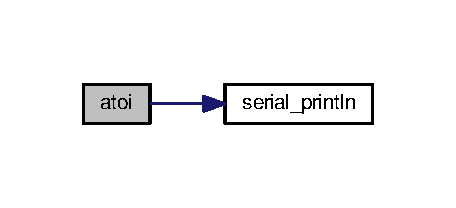
\includegraphics[width=219pt]{string_8c_a30670a60464f77af17dfb353353d6df8_cgraph}
\end{center}
\end{figure}




Here is the caller graph for this function\+:
\nopagebreak
\begin{figure}[H]
\begin{center}
\leavevmode
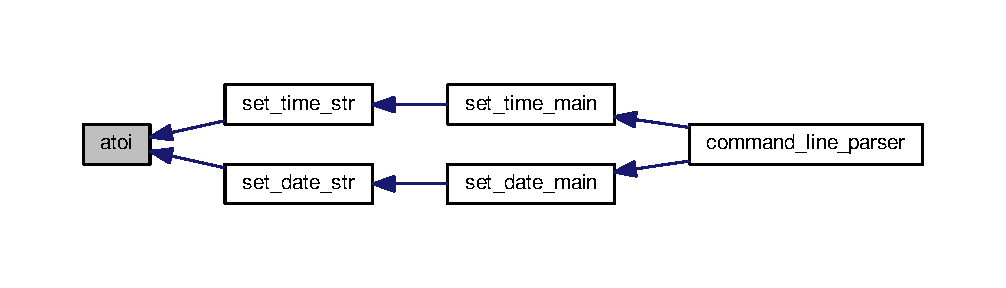
\includegraphics[width=350pt]{string_8c_a30670a60464f77af17dfb353353d6df8_icgraph}
\end{center}
\end{figure}


\index{string.\+c@{string.\+c}!isspace@{isspace}}
\index{isspace@{isspace}!string.\+c@{string.\+c}}
\subsubsection[{\texorpdfstring{isspace(const char $\ast$c)}{isspace(const char *c)}}]{\setlength{\rightskip}{0pt plus 5cm}int isspace (
\begin{DoxyParamCaption}
\item[{const char $\ast$}]{c}
\end{DoxyParamCaption}
)}\hypertarget{string_8c_a0f3d37d605e9e6d4fc1853ff9d4b91bf}{}\label{string_8c_a0f3d37d605e9e6d4fc1853ff9d4b91bf}
\index{string.\+c@{string.\+c}!memset@{memset}}
\index{memset@{memset}!string.\+c@{string.\+c}}
\subsubsection[{\texorpdfstring{memset(void $\ast$s, int c, size\+\_\+t n)}{memset(void *s, int c, size_t n)}}]{\setlength{\rightskip}{0pt plus 5cm}void$\ast$ memset (
\begin{DoxyParamCaption}
\item[{void $\ast$}]{s, }
\item[{int}]{c, }
\item[{size\+\_\+t}]{n}
\end{DoxyParamCaption}
)}\hypertarget{string_8c_ace6ee45c30e71865e6eb635200379db9}{}\label{string_8c_ace6ee45c30e71865e6eb635200379db9}


Here is the caller graph for this function\+:
\nopagebreak
\begin{figure}[H]
\begin{center}
\leavevmode
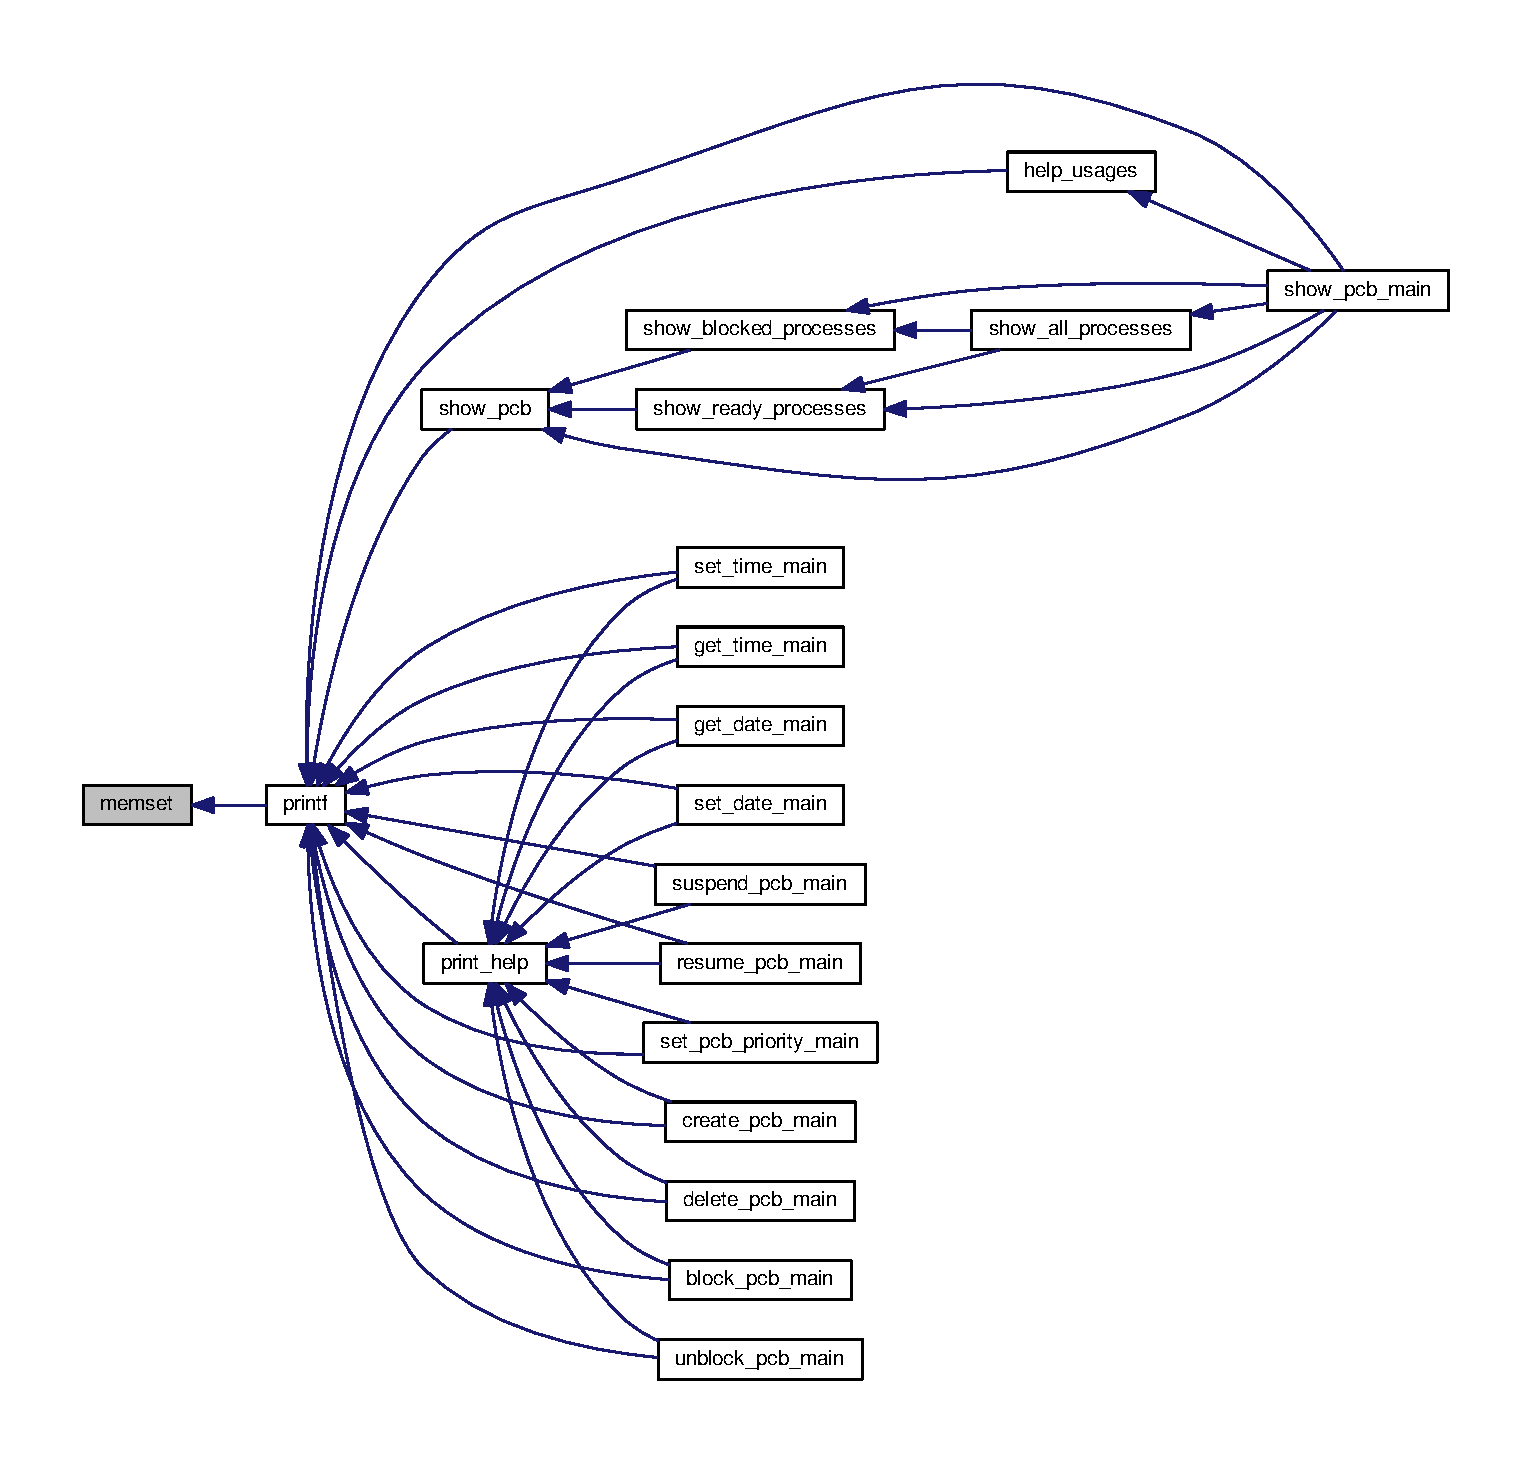
\includegraphics[width=350pt]{string_8c_ace6ee45c30e71865e6eb635200379db9_icgraph}
\end{center}
\end{figure}


\index{string.\+c@{string.\+c}!printf@{printf}}
\index{printf@{printf}!string.\+c@{string.\+c}}
\subsubsection[{\texorpdfstring{printf(const char $\ast$format,...)}{printf(const char *format,...)}}]{\setlength{\rightskip}{0pt plus 5cm}int printf (
\begin{DoxyParamCaption}
\item[{const char $\ast$}]{format, }
\item[{}]{...}
\end{DoxyParamCaption}
)}\hypertarget{string_8c_a98631211a4a8aee62f572375d5b637be}{}\label{string_8c_a98631211a4a8aee62f572375d5b637be}


Here is the call graph for this function\+:\nopagebreak
\begin{figure}[H]
\begin{center}
\leavevmode
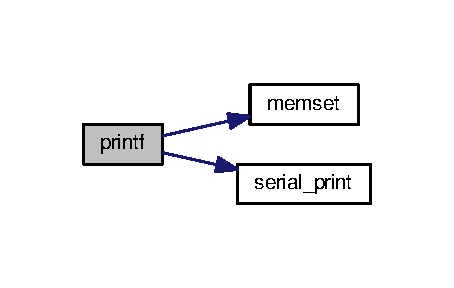
\includegraphics[width=218pt]{string_8c_a98631211a4a8aee62f572375d5b637be_cgraph}
\end{center}
\end{figure}




Here is the caller graph for this function\+:
\nopagebreak
\begin{figure}[H]
\begin{center}
\leavevmode
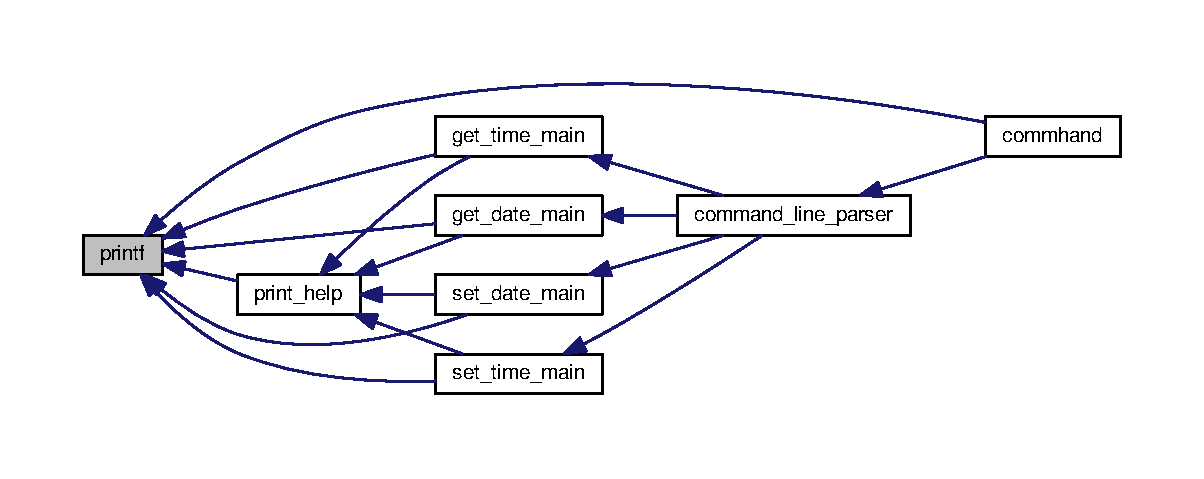
\includegraphics[width=350pt]{string_8c_a98631211a4a8aee62f572375d5b637be_icgraph}
\end{center}
\end{figure}


\index{string.\+c@{string.\+c}!sprintf@{sprintf}}
\index{sprintf@{sprintf}!string.\+c@{string.\+c}}
\subsubsection[{\texorpdfstring{sprintf(char $\ast$str, const char $\ast$format,...)}{sprintf(char *str, const char *format,...)}}]{\setlength{\rightskip}{0pt plus 5cm}int sprintf (
\begin{DoxyParamCaption}
\item[{char $\ast$}]{str, }
\item[{const char $\ast$}]{format, }
\item[{}]{...}
\end{DoxyParamCaption}
)}\hypertarget{string_8c_a3082155ec11e7229f7a20439b31a169e}{}\label{string_8c_a3082155ec11e7229f7a20439b31a169e}
\index{string.\+c@{string.\+c}!strcat@{strcat}}
\index{strcat@{strcat}!string.\+c@{string.\+c}}
\subsubsection[{\texorpdfstring{strcat(char $\ast$s1, const char $\ast$s2)}{strcat(char *s1, const char *s2)}}]{\setlength{\rightskip}{0pt plus 5cm}char$\ast$ strcat (
\begin{DoxyParamCaption}
\item[{char $\ast$}]{s1, }
\item[{const char $\ast$}]{s2}
\end{DoxyParamCaption}
)}\hypertarget{string_8c_a8908188ae9fc2f05d993257ef001d553}{}\label{string_8c_a8908188ae9fc2f05d993257ef001d553}


Here is the caller graph for this function\+:
\nopagebreak
\begin{figure}[H]
\begin{center}
\leavevmode
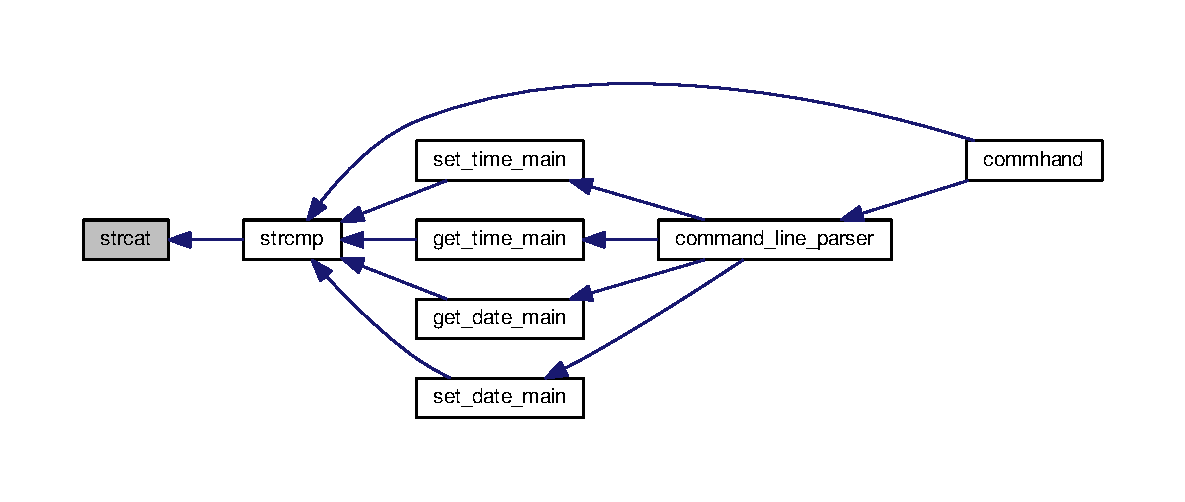
\includegraphics[width=350pt]{string_8c_a8908188ae9fc2f05d993257ef001d553_icgraph}
\end{center}
\end{figure}


\index{string.\+c@{string.\+c}!strcmp@{strcmp}}
\index{strcmp@{strcmp}!string.\+c@{string.\+c}}
\subsubsection[{\texorpdfstring{strcmp(const char $\ast$s1, const char $\ast$s2)}{strcmp(const char *s1, const char *s2)}}]{\setlength{\rightskip}{0pt plus 5cm}int strcmp (
\begin{DoxyParamCaption}
\item[{const char $\ast$}]{s1, }
\item[{const char $\ast$}]{s2}
\end{DoxyParamCaption}
)}\hypertarget{string_8c_a11bd144d7d44914099a3aeddf1c8567d}{}\label{string_8c_a11bd144d7d44914099a3aeddf1c8567d}


Here is the call graph for this function\+:\nopagebreak
\begin{figure}[H]
\begin{center}
\leavevmode
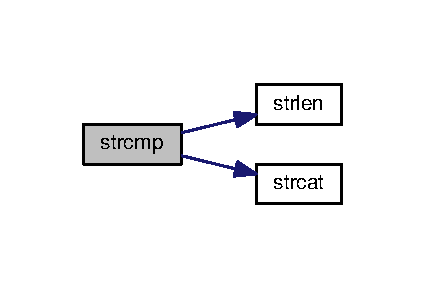
\includegraphics[width=204pt]{string_8c_a11bd144d7d44914099a3aeddf1c8567d_cgraph}
\end{center}
\end{figure}




Here is the caller graph for this function\+:
\nopagebreak
\begin{figure}[H]
\begin{center}
\leavevmode
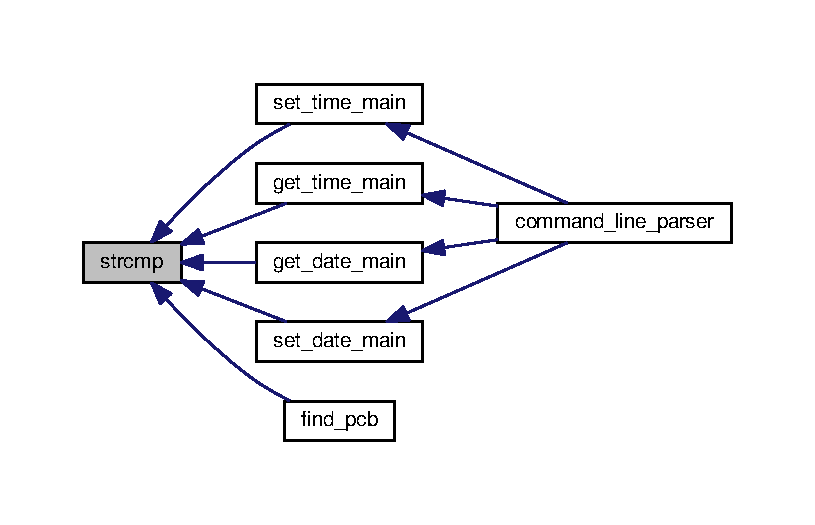
\includegraphics[width=350pt]{string_8c_a11bd144d7d44914099a3aeddf1c8567d_icgraph}
\end{center}
\end{figure}


\index{string.\+c@{string.\+c}!strcpy@{strcpy}}
\index{strcpy@{strcpy}!string.\+c@{string.\+c}}
\subsubsection[{\texorpdfstring{strcpy(char $\ast$s1, const char $\ast$s2)}{strcpy(char *s1, const char *s2)}}]{\setlength{\rightskip}{0pt plus 5cm}char$\ast$ strcpy (
\begin{DoxyParamCaption}
\item[{char $\ast$}]{s1, }
\item[{const char $\ast$}]{s2}
\end{DoxyParamCaption}
)}\hypertarget{string_8c_a1eb9cae61e6a6282c28dbc298ef7297e}{}\label{string_8c_a1eb9cae61e6a6282c28dbc298ef7297e}


Here is the caller graph for this function\+:
\nopagebreak
\begin{figure}[H]
\begin{center}
\leavevmode
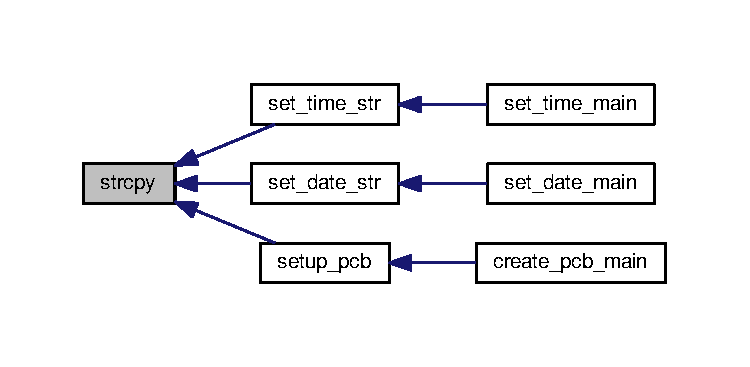
\includegraphics[width=350pt]{string_8c_a1eb9cae61e6a6282c28dbc298ef7297e_icgraph}
\end{center}
\end{figure}


\index{string.\+c@{string.\+c}!strlen@{strlen}}
\index{strlen@{strlen}!string.\+c@{string.\+c}}
\subsubsection[{\texorpdfstring{strlen(const char $\ast$s)}{strlen(const char *s)}}]{\setlength{\rightskip}{0pt plus 5cm}int strlen (
\begin{DoxyParamCaption}
\item[{const char $\ast$}]{s}
\end{DoxyParamCaption}
)}\hypertarget{string_8c_a2dee044e4e667b5b789b493abd21cfa4}{}\label{string_8c_a2dee044e4e667b5b789b493abd21cfa4}


Here is the caller graph for this function\+:
\nopagebreak
\begin{figure}[H]
\begin{center}
\leavevmode
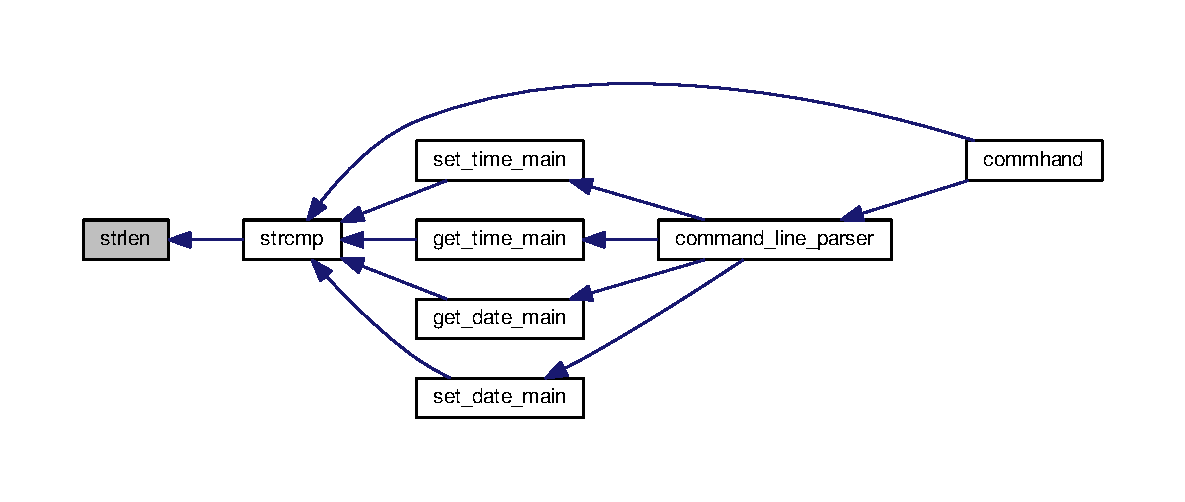
\includegraphics[width=350pt]{string_8c_a2dee044e4e667b5b789b493abd21cfa4_icgraph}
\end{center}
\end{figure}


\index{string.\+c@{string.\+c}!strtok@{strtok}}
\index{strtok@{strtok}!string.\+c@{string.\+c}}
\subsubsection[{\texorpdfstring{strtok(char $\ast$s1, const char $\ast$s2)}{strtok(char *s1, const char *s2)}}]{\setlength{\rightskip}{0pt plus 5cm}char$\ast$ strtok (
\begin{DoxyParamCaption}
\item[{char $\ast$}]{s1, }
\item[{const char $\ast$}]{s2}
\end{DoxyParamCaption}
)}\hypertarget{string_8c_af1a867dcea42fc1215d0eddf19283ef3}{}\label{string_8c_af1a867dcea42fc1215d0eddf19283ef3}


Here is the caller graph for this function\+:
\nopagebreak
\begin{figure}[H]
\begin{center}
\leavevmode
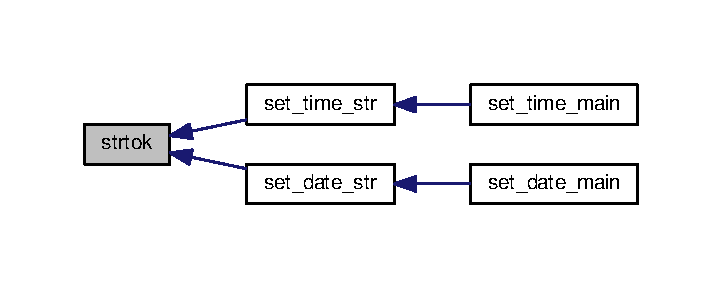
\includegraphics[width=350pt]{string_8c_af1a867dcea42fc1215d0eddf19283ef3_icgraph}
\end{center}
\end{figure}



\hypertarget{errno_8h}{\section{modules/errno.h File Reference}
\label{errno_8h}\index{modules/errno.\-h@{modules/errno.\-h}}
}


This file contains the type of errors. The error can be from invalid paramter passed to a function, or invalid input format.  


This graph shows which files directly or indirectly include this file\-:\nopagebreak
\begin{figure}[H]
\begin{center}
\leavevmode
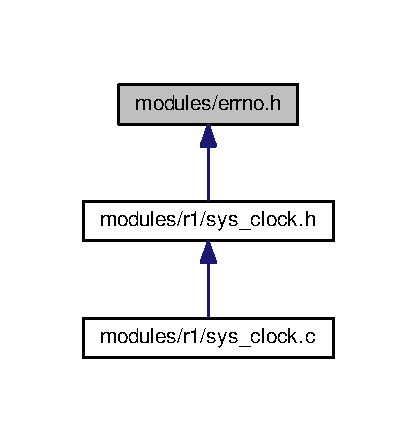
\includegraphics[width=350pt]{errno_8h__dep__incl}
\end{center}
\end{figure}
\subsection*{Macros}
\begin{DoxyCompactItemize}
\item 
\#define \hyperlink{errno_8h_a910656a3ce04eecb0e4479fd35d343fb}{E\-\_\-\-N\-O\-E\-R\-R\-O\-R}~0
\item 
\#define \hyperlink{errno_8h_ad38311f7eadb9042f7c98dd31ffc69c3}{E\-\_\-\-I\-N\-V\-P\-A\-R\-A}~1
\item 
\#define \hyperlink{errno_8h_a17ad8897d139d58bb84714b2e7861ba2}{E\-\_\-\-I\-N\-V\-S\-T\-R\-F}~2
\item 
\#define \hyperlink{errno_8h_a5273e7742dd7c18937e5191b8070f08f}{E\-\_\-\-I\-N\-V\-U\-S\-R\-I}~3
\item 
\#define \hyperlink{errno_8h_a7fcfdab3c40ca9d8eb249d636908c3fd}{E\-\_\-\-F\-R\-E\-E\-M\-E\-M}~4
\begin{DoxyCompactList}\small\item\em Error we cannot actually free the memory space since the student\-\_\-free had not been implemented before R5. \end{DoxyCompactList}\item 
\#define \hyperlink{errno_8h_a97fcdfde06438bcf94181400389bd7b9}{E\-\_\-\-N\-U\-L\-L\-\_\-\-P\-T\-R}~5
\begin{DoxyCompactList}\small\item\em A N\-U\-L\-L Pointer Error. \end{DoxyCompactList}\item 
\#define \hyperlink{errno_8h_af40255ba5e6a1e879803d699b4393cac}{E\-\_\-\-P\-R\-O\-G\-E\-R\-R}~99
\end{DoxyCompactItemize}
\subsection*{Typedefs}
\begin{Indent}{\bf error\-\_\-t.}\par
{\em The datetype that holds the error code. }\begin{DoxyCompactItemize}
\item 
typedef unsigned int \hyperlink{errno_8h_aafbeb34410283829794b35fedafeb369}{error\-\_\-t}
\end{DoxyCompactItemize}
\end{Indent}


\subsection{Detailed Description}
This file contains the type of errors. The error can be from invalid paramter passed to a function, or invalid input format. \begin{DoxyAuthor}{Author}
Thunder Krakens 
\end{DoxyAuthor}
\begin{DoxyDate}{Date}
February 7nd, 2016 
\end{DoxyDate}
\begin{DoxyVersion}{Version}
R2 
\end{DoxyVersion}


\subsection{Macro Definition Documentation}
\hypertarget{errno_8h_a7fcfdab3c40ca9d8eb249d636908c3fd}{\index{errno.\-h@{errno.\-h}!E\-\_\-\-F\-R\-E\-E\-M\-E\-M@{E\-\_\-\-F\-R\-E\-E\-M\-E\-M}}
\index{E\-\_\-\-F\-R\-E\-E\-M\-E\-M@{E\-\_\-\-F\-R\-E\-E\-M\-E\-M}!errno.h@{errno.\-h}}
\subsubsection[{E\-\_\-\-F\-R\-E\-E\-M\-E\-M}]{\setlength{\rightskip}{0pt plus 5cm}\#define E\-\_\-\-F\-R\-E\-E\-M\-E\-M~4}}\label{errno_8h_a7fcfdab3c40ca9d8eb249d636908c3fd}


Error we cannot actually free the memory space since the student\-\_\-free had not been implemented before R5. 

\hypertarget{errno_8h_ad38311f7eadb9042f7c98dd31ffc69c3}{\index{errno.\-h@{errno.\-h}!E\-\_\-\-I\-N\-V\-P\-A\-R\-A@{E\-\_\-\-I\-N\-V\-P\-A\-R\-A}}
\index{E\-\_\-\-I\-N\-V\-P\-A\-R\-A@{E\-\_\-\-I\-N\-V\-P\-A\-R\-A}!errno.h@{errno.\-h}}
\subsubsection[{E\-\_\-\-I\-N\-V\-P\-A\-R\-A}]{\setlength{\rightskip}{0pt plus 5cm}\#define E\-\_\-\-I\-N\-V\-P\-A\-R\-A~1}}\label{errno_8h_ad38311f7eadb9042f7c98dd31ffc69c3}
\hypertarget{errno_8h_a17ad8897d139d58bb84714b2e7861ba2}{\index{errno.\-h@{errno.\-h}!E\-\_\-\-I\-N\-V\-S\-T\-R\-F@{E\-\_\-\-I\-N\-V\-S\-T\-R\-F}}
\index{E\-\_\-\-I\-N\-V\-S\-T\-R\-F@{E\-\_\-\-I\-N\-V\-S\-T\-R\-F}!errno.h@{errno.\-h}}
\subsubsection[{E\-\_\-\-I\-N\-V\-S\-T\-R\-F}]{\setlength{\rightskip}{0pt plus 5cm}\#define E\-\_\-\-I\-N\-V\-S\-T\-R\-F~2}}\label{errno_8h_a17ad8897d139d58bb84714b2e7861ba2}
\hypertarget{errno_8h_a5273e7742dd7c18937e5191b8070f08f}{\index{errno.\-h@{errno.\-h}!E\-\_\-\-I\-N\-V\-U\-S\-R\-I@{E\-\_\-\-I\-N\-V\-U\-S\-R\-I}}
\index{E\-\_\-\-I\-N\-V\-U\-S\-R\-I@{E\-\_\-\-I\-N\-V\-U\-S\-R\-I}!errno.h@{errno.\-h}}
\subsubsection[{E\-\_\-\-I\-N\-V\-U\-S\-R\-I}]{\setlength{\rightskip}{0pt plus 5cm}\#define E\-\_\-\-I\-N\-V\-U\-S\-R\-I~3}}\label{errno_8h_a5273e7742dd7c18937e5191b8070f08f}
\hypertarget{errno_8h_a910656a3ce04eecb0e4479fd35d343fb}{\index{errno.\-h@{errno.\-h}!E\-\_\-\-N\-O\-E\-R\-R\-O\-R@{E\-\_\-\-N\-O\-E\-R\-R\-O\-R}}
\index{E\-\_\-\-N\-O\-E\-R\-R\-O\-R@{E\-\_\-\-N\-O\-E\-R\-R\-O\-R}!errno.h@{errno.\-h}}
\subsubsection[{E\-\_\-\-N\-O\-E\-R\-R\-O\-R}]{\setlength{\rightskip}{0pt plus 5cm}\#define E\-\_\-\-N\-O\-E\-R\-R\-O\-R~0}}\label{errno_8h_a910656a3ce04eecb0e4479fd35d343fb}
\hypertarget{errno_8h_a97fcdfde06438bcf94181400389bd7b9}{\index{errno.\-h@{errno.\-h}!E\-\_\-\-N\-U\-L\-L\-\_\-\-P\-T\-R@{E\-\_\-\-N\-U\-L\-L\-\_\-\-P\-T\-R}}
\index{E\-\_\-\-N\-U\-L\-L\-\_\-\-P\-T\-R@{E\-\_\-\-N\-U\-L\-L\-\_\-\-P\-T\-R}!errno.h@{errno.\-h}}
\subsubsection[{E\-\_\-\-N\-U\-L\-L\-\_\-\-P\-T\-R}]{\setlength{\rightskip}{0pt plus 5cm}\#define E\-\_\-\-N\-U\-L\-L\-\_\-\-P\-T\-R~5}}\label{errno_8h_a97fcdfde06438bcf94181400389bd7b9}


A N\-U\-L\-L Pointer Error. 

\hypertarget{errno_8h_af40255ba5e6a1e879803d699b4393cac}{\index{errno.\-h@{errno.\-h}!E\-\_\-\-P\-R\-O\-G\-E\-R\-R@{E\-\_\-\-P\-R\-O\-G\-E\-R\-R}}
\index{E\-\_\-\-P\-R\-O\-G\-E\-R\-R@{E\-\_\-\-P\-R\-O\-G\-E\-R\-R}!errno.h@{errno.\-h}}
\subsubsection[{E\-\_\-\-P\-R\-O\-G\-E\-R\-R}]{\setlength{\rightskip}{0pt plus 5cm}\#define E\-\_\-\-P\-R\-O\-G\-E\-R\-R~99}}\label{errno_8h_af40255ba5e6a1e879803d699b4393cac}


\subsection{Typedef Documentation}
\hypertarget{errno_8h_aafbeb34410283829794b35fedafeb369}{\index{errno.\-h@{errno.\-h}!error\-\_\-t@{error\-\_\-t}}
\index{error\-\_\-t@{error\-\_\-t}!errno.h@{errno.\-h}}
\subsubsection[{error\-\_\-t}]{\setlength{\rightskip}{0pt plus 5cm}typedef unsigned int {\bf error\-\_\-t}}}\label{errno_8h_aafbeb34410283829794b35fedafeb369}

\hypertarget{r1_8c}{}\section{modules/r1/r1.c File Reference}
\label{r1_8c}\index{modules/r1/r1.\+c@{modules/r1/r1.\+c}}


The main code file for Module R1.  


{\ttfamily \#include \char`\"{}r1.\+h\char`\"{}}\\*
{\ttfamily \#include \char`\"{}../mpx\+\_\+supt.\+h\char`\"{}}\\*
{\ttfamily \#include \char`\"{}sys\+\_\+clock.\+h\char`\"{}}\\*
{\ttfamily \#include $<$string.\+h$>$}\\*
{\ttfamily \#include $<$core/serial.\+h$>$}\\*
{\ttfamily \#include $<$core/io.\+h$>$}\\*
\subsection*{Macros}
\begin{DoxyCompactItemize}
\item 
\#define {\bfseries U\+S\+E\+R\+\_\+\+I\+N\+P\+U\+T\+\_\+\+B\+U\+F\+F\+E\+R\+\_\+\+S\+I\+ZE}~1000\hypertarget{r1_8c_abcc7a443a9849435cd308e774dd0c8de}{}\label{r1_8c_abcc7a443a9849435cd308e774dd0c8de}

\item 
\#define {\bfseries M\+A\+X\+\_\+\+A\+R\+GC}~50\hypertarget{r1_8c_ae1da50c0d24fa0390a6c287d6cb4befe}{}\label{r1_8c_ae1da50c0d24fa0390a6c287d6cb4befe}

\item 
\#define {\bfseries M\+O\+D\+\_\+\+V\+E\+R\+S\+I\+ON}~\char`\"{}R1\char`\"{}\hypertarget{r1_8c_a88a929d879ebd5f0d64773050f62aef5}{}\label{r1_8c_a88a929d879ebd5f0d64773050f62aef5}

\item 
\#define {\bfseries C\+O\+M\+P\+L\+E\+T\+I\+ON}~\char`\"{}02/05/2016\char`\"{}\hypertarget{r1_8c_afc29c35952a1ce914016dbfa4b91c2aa}{}\label{r1_8c_afc29c35952a1ce914016dbfa4b91c2aa}

\end{DoxyCompactItemize}
\subsection*{Enumerations}
\begin{DoxyCompactItemize}
\item 
enum \hyperlink{r1_8c_abb950b1df1e3f5562228a4eae8ebb925}{Command\+Paser\+Stat} \{ {\bfseries Not\+Writing}, 
{\bfseries Normal\+Writing}, 
{\bfseries Double\+Quote\+Writing}, 
{\bfseries Single\+Quote\+Writing}
 \}\begin{DoxyCompactList}\small\item\em Name\+: Command\+Parser\+Stat. \end{DoxyCompactList}
\end{DoxyCompactItemize}
\subsection*{Functions}
\begin{DoxyCompactItemize}
\item 
int \hyperlink{r1_8c_a14d85617242501c323a203ee196d3efa}{commhand} ()
\begin{DoxyCompactList}\small\item\em Name\+: commhand. \end{DoxyCompactList}\item 
void \hyperlink{r1_8c_adb6b307c73bca25d17aa7683e14fea16}{command\+\_\+line\+\_\+parser} (const char $\ast$Cmd\+Str, int $\ast$argc, char $\ast$$\ast$argv, const int Max\+Arg\+Num, const int Max\+Str\+Len)
\begin{DoxyCompactList}\small\item\em Name\+: command\+\_\+line\+\_\+parser. \end{DoxyCompactList}\end{DoxyCompactItemize}


\subsection{Detailed Description}
The main code file for Module R1. 

\begin{DoxyAuthor}{Author}
Thunder Krakens 
\end{DoxyAuthor}
\begin{DoxyDate}{Date}
February 2nd, 2016 
\end{DoxyDate}
\begin{DoxyVersion}{Version}
R1
\end{DoxyVersion}
This file contains setdate, getdate, settime, gettime, help functions, commandhander and command line parser 

\subsection{Enumeration Type Documentation}
\index{r1.\+c@{r1.\+c}!Command\+Paser\+Stat@{Command\+Paser\+Stat}}
\index{Command\+Paser\+Stat@{Command\+Paser\+Stat}!r1.\+c@{r1.\+c}}
\subsubsection[{\texorpdfstring{Command\+Paser\+Stat}{CommandPaserStat}}]{\setlength{\rightskip}{0pt plus 5cm}enum {\bf Command\+Paser\+Stat}}\hypertarget{r1_8c_abb950b1df1e3f5562228a4eae8ebb925}{}\label{r1_8c_abb950b1df1e3f5562228a4eae8ebb925}


Name\+: Command\+Parser\+Stat. 

Description\+: The stats of the command parser 

\subsection{Function Documentation}
\index{r1.\+c@{r1.\+c}!command\+\_\+line\+\_\+parser@{command\+\_\+line\+\_\+parser}}
\index{command\+\_\+line\+\_\+parser@{command\+\_\+line\+\_\+parser}!r1.\+c@{r1.\+c}}
\subsubsection[{\texorpdfstring{command\+\_\+line\+\_\+parser(const char $\ast$\+Cmd\+Str, int $\ast$argc, char $\ast$$\ast$argv, const int Max\+Arg\+Num, const int Max\+Str\+Len)}{command_line_parser(const char *CmdStr, int *argc, char **argv, const int MaxArgNum, const int MaxStrLen)}}]{\setlength{\rightskip}{0pt plus 5cm}void command\+\_\+line\+\_\+parser (
\begin{DoxyParamCaption}
\item[{const char $\ast$}]{Cmd\+Str, }
\item[{int $\ast$}]{argc, }
\item[{char $\ast$$\ast$}]{argv, }
\item[{const int}]{Max\+Arg\+Num, }
\item[{const int}]{Max\+Str\+Len}
\end{DoxyParamCaption}
)}\hypertarget{r1_8c_adb6b307c73bca25d17aa7683e14fea16}{}\label{r1_8c_adb6b307c73bca25d17aa7683e14fea16}


Name\+: command\+\_\+line\+\_\+parser. 

Description\+: Splits the complete command line into tokens by space, single quote, or double quote.


\begin{DoxyParams}{Parameters}
{\em Cmd\+Str} & -\/ The complete input command. \\
\hline
{\em argc} & -\/ The number of tokens found. \\
\hline
{\em argv} & -\/ The array of tokens. \\
\hline
{\em Max\+Arg\+Num} & -\/ The maximum number of tokens that array can hold. \\
\hline
{\em Max\+Str\+Len} & -\/ The maximum length of each token that string can hold.\\
\hline
\end{DoxyParams}
\begin{DoxyReturn}{Returns}
void 
\end{DoxyReturn}
\index{r1.\+c@{r1.\+c}!commhand@{commhand}}
\index{commhand@{commhand}!r1.\+c@{r1.\+c}}
\subsubsection[{\texorpdfstring{commhand()}{commhand()}}]{\setlength{\rightskip}{0pt plus 5cm}int commhand (
\begin{DoxyParamCaption}
{}
\end{DoxyParamCaption}
)}\hypertarget{r1_8c_a14d85617242501c323a203ee196d3efa}{}\label{r1_8c_a14d85617242501c323a203ee196d3efa}


Name\+: commhand. 

Description\+: Accepts and handles commands from the user. 
\begin{DoxyParams}{Parameters}
{\em User} & input \\
\hline
\end{DoxyParams}
\begin{DoxyReturn}{Returns}
0 
\end{DoxyReturn}

\hypertarget{r1_8h}{}\section{modules/r1/r1.h File Reference}
\label{r1_8h}\index{modules/r1/r1.\+h@{modules/r1/r1.\+h}}


The commandhander and functions associations for Module R1.  


This graph shows which files directly or indirectly include this file\+:\nopagebreak
\begin{figure}[H]
\begin{center}
\leavevmode
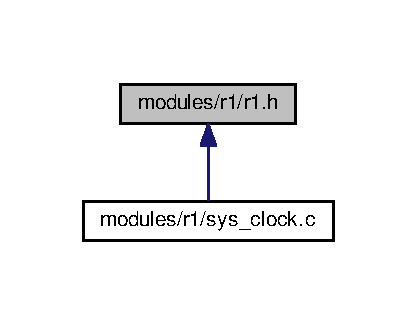
\includegraphics[width=302pt]{r1_8h__dep__incl}
\end{center}
\end{figure}
\subsection*{Macros}
\begin{DoxyCompactItemize}
\item 
\#define \hyperlink{r1_8h_ae8a798ec5e0449028e485688e8241b5e}{H\+E\+LP}~0
\item 
\#define \hyperlink{r1_8h_a1c6d5de492ac61ad29aec7aa9a436bbf}{V\+E\+R\+S\+I\+ON}~1
\item 
\#define \hyperlink{r1_8h_ab1586d6a1539e7921374aeea8b907805}{G\+E\+T\+T\+I\+ME}~2
\item 
\#define \hyperlink{r1_8h_a27a942da2560b15dc5291c8f386c426a}{S\+E\+T\+T\+I\+ME}~3
\item 
\#define \hyperlink{r1_8h_a6ec5835e6ff9d5af0a3a1996746ee5b9}{G\+E\+T\+D\+A\+TE}~4
\item 
\#define \hyperlink{r1_8h_ac1f0ac55b810f16f95393b27e9780bf3}{S\+E\+T\+D\+A\+TE}~5
\item 
\#define \hyperlink{r1_8h_a3b61478edd7c1b25c8facd2907cf6c33}{S\+H\+U\+T\+D\+O\+WN}~6
\item 
\#define \hyperlink{r1_8h_a8e8928373d15397e25be8ecb76c727da}{N\+U\+M\+\_\+\+O\+F\+\_\+\+F\+U\+N\+C\+T\+I\+O\+NS}~7
\end{DoxyCompactItemize}
\subsection*{Functions}
\begin{Indent}{\bf commhand}\par
{\em Accepts and handles commands from the user.

\begin{DoxyReturn}{Returns}
0 
\end{DoxyReturn}
}\begin{DoxyCompactItemize}
\item 
int \hyperlink{r1_8h_a14d85617242501c323a203ee196d3efa}{commhand} ()
\end{DoxyCompactItemize}
\end{Indent}
\begin{Indent}{\bf command\+\_\+line\+\_\+parser}\par
{\em Splits the complete command line into tokens by space, single quote, or double quote.


\begin{DoxyParams}{Parameters}
{\em Cmd\+Str} & The complete input command. \\
\hline
{\em argc} & The number of tokens found. \\
\hline
{\em argv} & The array of tokens. \\
\hline
{\em Max\+Arg\+Num} & The maximum number of tokens that array can hold. \\
\hline
{\em Max\+Str\+Len} & The maximum length of each token that string can hold.\\
\hline
\end{DoxyParams}
\begin{DoxyReturn}{Returns}
void 
\end{DoxyReturn}
}\begin{DoxyCompactItemize}
\item 
void \hyperlink{r1_8h_adb6b307c73bca25d17aa7683e14fea16}{command\+\_\+line\+\_\+parser} (const char $\ast$Cmd\+Str, int $\ast$argc, char $\ast$$\ast$argv, const int Max\+Arg\+Num, const int Max\+Str\+Len)
\end{DoxyCompactItemize}
\end{Indent}
\begin{Indent}{\bf print\+\_\+help}\par
{\em prints the help message of a certain function that specified by the index number


\begin{DoxyParams}{Parameters}
{\em function\+\_\+index} & The index number of that function.\\
\hline
\end{DoxyParams}
\begin{DoxyReturn}{Returns}
void 
\end{DoxyReturn}
}\begin{DoxyCompactItemize}
\item 
void \hyperlink{r1_8h_ab5b36414d84437d45b388232a0dfa366}{print\+\_\+help} (const int function\+\_\+index)
\end{DoxyCompactItemize}
\end{Indent}


\subsection{Detailed Description}
The commandhander and functions associations for Module R1. 

\begin{DoxyAuthor}{Author}
Thunder Krakens 
\end{DoxyAuthor}
\begin{DoxyDate}{Date}
February 2nd, 2016 
\end{DoxyDate}
\begin{DoxyVersion}{Version}
R1 
\end{DoxyVersion}


\subsection{Macro Definition Documentation}
\index{r1.\+h@{r1.\+h}!G\+E\+T\+D\+A\+TE@{G\+E\+T\+D\+A\+TE}}
\index{G\+E\+T\+D\+A\+TE@{G\+E\+T\+D\+A\+TE}!r1.\+h@{r1.\+h}}
\subsubsection[{\texorpdfstring{G\+E\+T\+D\+A\+TE}{GETDATE}}]{\setlength{\rightskip}{0pt plus 5cm}\#define G\+E\+T\+D\+A\+TE~4}\hypertarget{r1_8h_a6ec5835e6ff9d5af0a3a1996746ee5b9}{}\label{r1_8h_a6ec5835e6ff9d5af0a3a1996746ee5b9}
\index{r1.\+h@{r1.\+h}!G\+E\+T\+T\+I\+ME@{G\+E\+T\+T\+I\+ME}}
\index{G\+E\+T\+T\+I\+ME@{G\+E\+T\+T\+I\+ME}!r1.\+h@{r1.\+h}}
\subsubsection[{\texorpdfstring{G\+E\+T\+T\+I\+ME}{GETTIME}}]{\setlength{\rightskip}{0pt plus 5cm}\#define G\+E\+T\+T\+I\+ME~2}\hypertarget{r1_8h_ab1586d6a1539e7921374aeea8b907805}{}\label{r1_8h_ab1586d6a1539e7921374aeea8b907805}
\index{r1.\+h@{r1.\+h}!H\+E\+LP@{H\+E\+LP}}
\index{H\+E\+LP@{H\+E\+LP}!r1.\+h@{r1.\+h}}
\subsubsection[{\texorpdfstring{H\+E\+LP}{HELP}}]{\setlength{\rightskip}{0pt plus 5cm}\#define H\+E\+LP~0}\hypertarget{r1_8h_ae8a798ec5e0449028e485688e8241b5e}{}\label{r1_8h_ae8a798ec5e0449028e485688e8241b5e}
\index{r1.\+h@{r1.\+h}!N\+U\+M\+\_\+\+O\+F\+\_\+\+F\+U\+N\+C\+T\+I\+O\+NS@{N\+U\+M\+\_\+\+O\+F\+\_\+\+F\+U\+N\+C\+T\+I\+O\+NS}}
\index{N\+U\+M\+\_\+\+O\+F\+\_\+\+F\+U\+N\+C\+T\+I\+O\+NS@{N\+U\+M\+\_\+\+O\+F\+\_\+\+F\+U\+N\+C\+T\+I\+O\+NS}!r1.\+h@{r1.\+h}}
\subsubsection[{\texorpdfstring{N\+U\+M\+\_\+\+O\+F\+\_\+\+F\+U\+N\+C\+T\+I\+O\+NS}{NUM_OF_FUNCTIONS}}]{\setlength{\rightskip}{0pt plus 5cm}\#define N\+U\+M\+\_\+\+O\+F\+\_\+\+F\+U\+N\+C\+T\+I\+O\+NS~7}\hypertarget{r1_8h_a8e8928373d15397e25be8ecb76c727da}{}\label{r1_8h_a8e8928373d15397e25be8ecb76c727da}
\index{r1.\+h@{r1.\+h}!S\+E\+T\+D\+A\+TE@{S\+E\+T\+D\+A\+TE}}
\index{S\+E\+T\+D\+A\+TE@{S\+E\+T\+D\+A\+TE}!r1.\+h@{r1.\+h}}
\subsubsection[{\texorpdfstring{S\+E\+T\+D\+A\+TE}{SETDATE}}]{\setlength{\rightskip}{0pt plus 5cm}\#define S\+E\+T\+D\+A\+TE~5}\hypertarget{r1_8h_ac1f0ac55b810f16f95393b27e9780bf3}{}\label{r1_8h_ac1f0ac55b810f16f95393b27e9780bf3}
\index{r1.\+h@{r1.\+h}!S\+E\+T\+T\+I\+ME@{S\+E\+T\+T\+I\+ME}}
\index{S\+E\+T\+T\+I\+ME@{S\+E\+T\+T\+I\+ME}!r1.\+h@{r1.\+h}}
\subsubsection[{\texorpdfstring{S\+E\+T\+T\+I\+ME}{SETTIME}}]{\setlength{\rightskip}{0pt plus 5cm}\#define S\+E\+T\+T\+I\+ME~3}\hypertarget{r1_8h_a27a942da2560b15dc5291c8f386c426a}{}\label{r1_8h_a27a942da2560b15dc5291c8f386c426a}
\index{r1.\+h@{r1.\+h}!S\+H\+U\+T\+D\+O\+WN@{S\+H\+U\+T\+D\+O\+WN}}
\index{S\+H\+U\+T\+D\+O\+WN@{S\+H\+U\+T\+D\+O\+WN}!r1.\+h@{r1.\+h}}
\subsubsection[{\texorpdfstring{S\+H\+U\+T\+D\+O\+WN}{SHUTDOWN}}]{\setlength{\rightskip}{0pt plus 5cm}\#define S\+H\+U\+T\+D\+O\+WN~6}\hypertarget{r1_8h_a3b61478edd7c1b25c8facd2907cf6c33}{}\label{r1_8h_a3b61478edd7c1b25c8facd2907cf6c33}
\index{r1.\+h@{r1.\+h}!V\+E\+R\+S\+I\+ON@{V\+E\+R\+S\+I\+ON}}
\index{V\+E\+R\+S\+I\+ON@{V\+E\+R\+S\+I\+ON}!r1.\+h@{r1.\+h}}
\subsubsection[{\texorpdfstring{V\+E\+R\+S\+I\+ON}{VERSION}}]{\setlength{\rightskip}{0pt plus 5cm}\#define V\+E\+R\+S\+I\+ON~1}\hypertarget{r1_8h_a1c6d5de492ac61ad29aec7aa9a436bbf}{}\label{r1_8h_a1c6d5de492ac61ad29aec7aa9a436bbf}


\subsection{Function Documentation}
\index{r1.\+h@{r1.\+h}!command\+\_\+line\+\_\+parser@{command\+\_\+line\+\_\+parser}}
\index{command\+\_\+line\+\_\+parser@{command\+\_\+line\+\_\+parser}!r1.\+h@{r1.\+h}}
\subsubsection[{\texorpdfstring{command\+\_\+line\+\_\+parser(const char $\ast$\+Cmd\+Str, int $\ast$argc, char $\ast$$\ast$argv, const int Max\+Arg\+Num, const int Max\+Str\+Len)}{command_line_parser(const char *CmdStr, int *argc, char **argv, const int MaxArgNum, const int MaxStrLen)}}]{\setlength{\rightskip}{0pt plus 5cm}void command\+\_\+line\+\_\+parser (
\begin{DoxyParamCaption}
\item[{const char $\ast$}]{Cmd\+Str, }
\item[{int $\ast$}]{argc, }
\item[{char $\ast$$\ast$}]{argv, }
\item[{const int}]{Max\+Arg\+Num, }
\item[{const int}]{Max\+Str\+Len}
\end{DoxyParamCaption}
)}\hypertarget{r1_8h_adb6b307c73bca25d17aa7683e14fea16}{}\label{r1_8h_adb6b307c73bca25d17aa7683e14fea16}


Here is the call graph for this function\+:\nopagebreak
\begin{figure}[H]
\begin{center}
\leavevmode
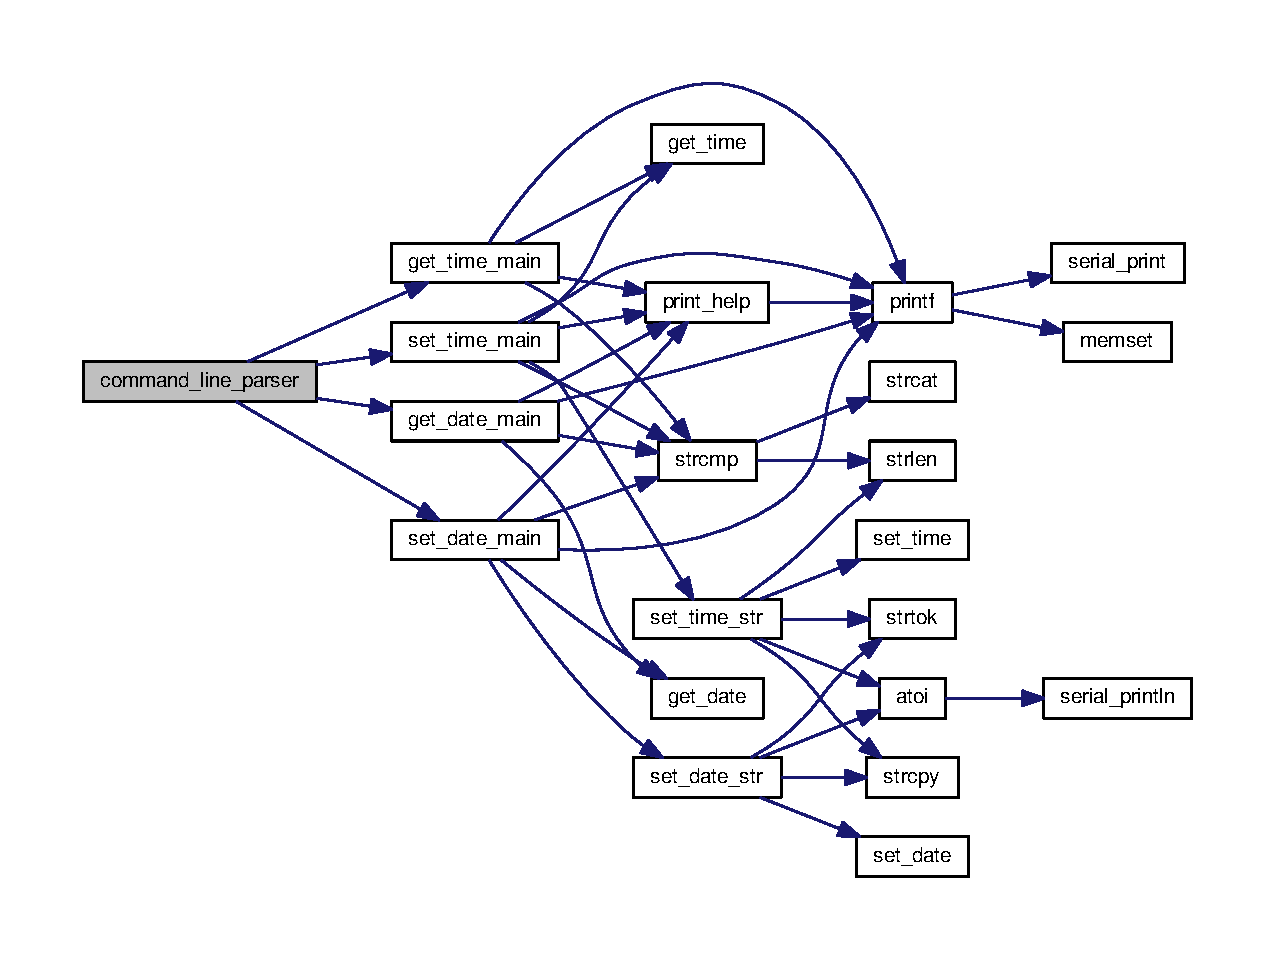
\includegraphics[width=350pt]{r1_8h_adb6b307c73bca25d17aa7683e14fea16_cgraph}
\end{center}
\end{figure}




Here is the caller graph for this function\+:\nopagebreak
\begin{figure}[H]
\begin{center}
\leavevmode
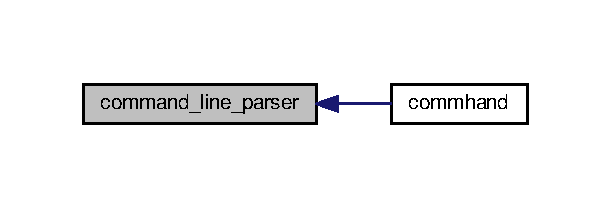
\includegraphics[width=293pt]{r1_8h_adb6b307c73bca25d17aa7683e14fea16_icgraph}
\end{center}
\end{figure}


\index{r1.\+h@{r1.\+h}!commhand@{commhand}}
\index{commhand@{commhand}!r1.\+h@{r1.\+h}}
\subsubsection[{\texorpdfstring{commhand()}{commhand()}}]{\setlength{\rightskip}{0pt plus 5cm}int commhand (
\begin{DoxyParamCaption}
{}
\end{DoxyParamCaption}
)}\hypertarget{r1_8h_a14d85617242501c323a203ee196d3efa}{}\label{r1_8h_a14d85617242501c323a203ee196d3efa}


Here is the call graph for this function\+:\nopagebreak
\begin{figure}[H]
\begin{center}
\leavevmode
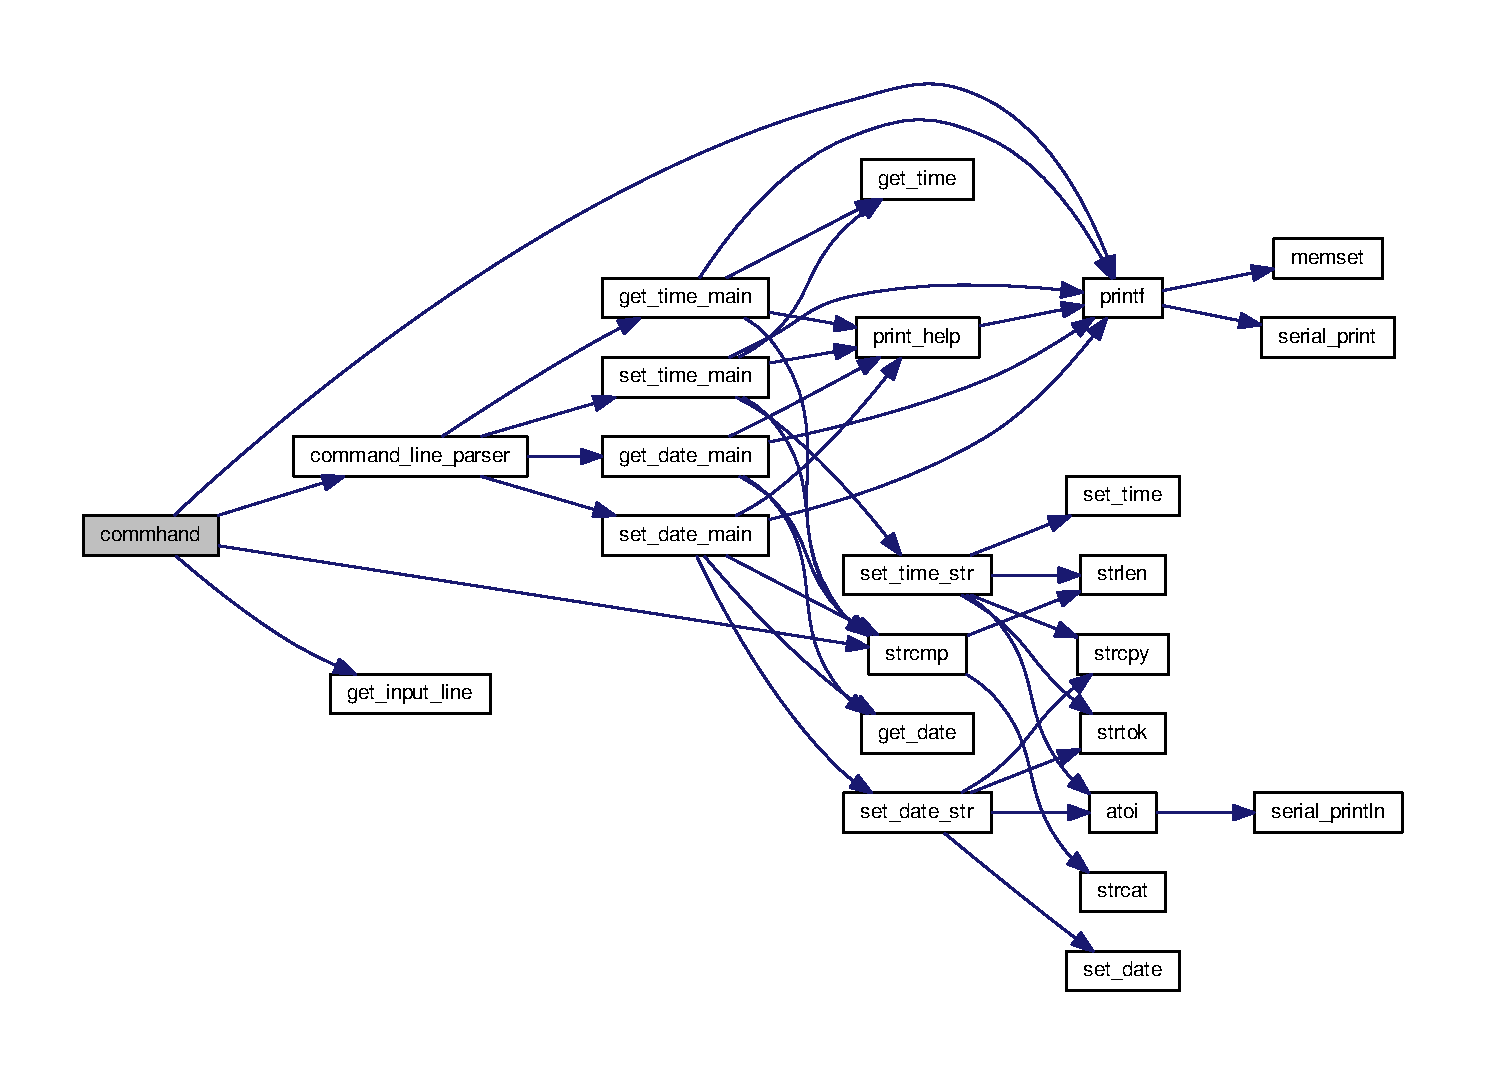
\includegraphics[width=350pt]{r1_8h_a14d85617242501c323a203ee196d3efa_cgraph}
\end{center}
\end{figure}


\index{r1.\+h@{r1.\+h}!print\+\_\+help@{print\+\_\+help}}
\index{print\+\_\+help@{print\+\_\+help}!r1.\+h@{r1.\+h}}
\subsubsection[{\texorpdfstring{print\+\_\+help(const int function\+\_\+index)}{print_help(const int function_index)}}]{\setlength{\rightskip}{0pt plus 5cm}void print\+\_\+help (
\begin{DoxyParamCaption}
\item[{const int}]{function\+\_\+index}
\end{DoxyParamCaption}
)}\hypertarget{r1_8h_ab5b36414d84437d45b388232a0dfa366}{}\label{r1_8h_ab5b36414d84437d45b388232a0dfa366}


Here is the call graph for this function\+:\nopagebreak
\begin{figure}[H]
\begin{center}
\leavevmode
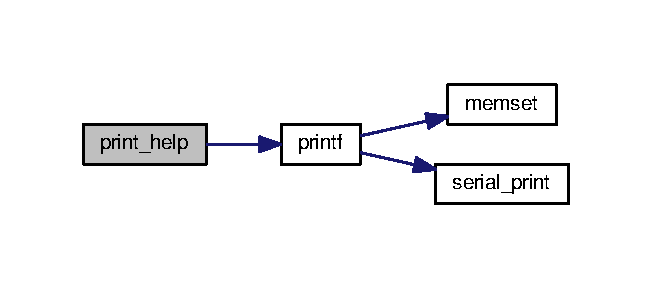
\includegraphics[width=313pt]{r1_8h_ab5b36414d84437d45b388232a0dfa366_cgraph}
\end{center}
\end{figure}




Here is the caller graph for this function\+:\nopagebreak
\begin{figure}[H]
\begin{center}
\leavevmode
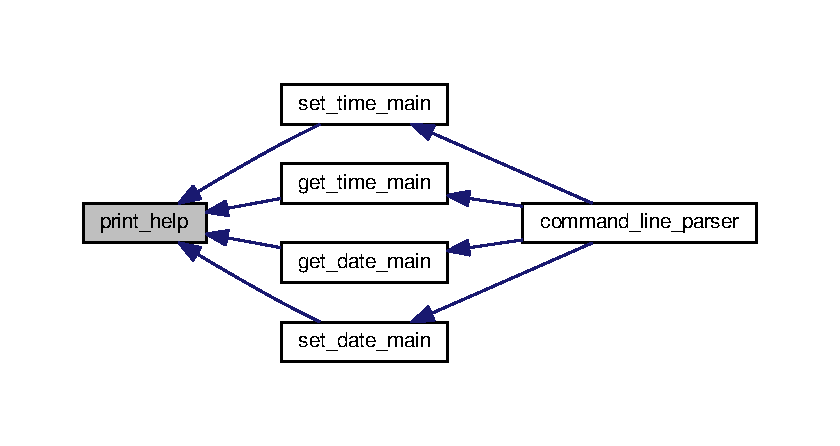
\includegraphics[width=350pt]{r1_8h_ab5b36414d84437d45b388232a0dfa366_icgraph}
\end{center}
\end{figure}



%--- End generated contents ---

% Index
\backmatter
\newpage
\phantomsection
\clearemptydoublepage
\addcontentsline{toc}{chapter}{Index}
\printindex

\end{document}
